%% RC-Gate -- Springer Nature (sn-jnl), single-column layout
\documentclass[pdflatex,sn-mathphys,Numbered]{sn-jnl}
\hypersetup{hypertexnames=false}

\usepackage{graphicx}%
\usepackage{multirow}%
\usepackage{amsmath,amssymb,amsfonts}%
\usepackage{amsthm}%
\usepackage{mathrsfs}%
\usepackage{xcolor}%
\usepackage{textcomp}%
\usepackage{manyfoot}%
\usepackage{booktabs}%
\usepackage{algorithm}%
\usepackage{algorithmicx}%
\usepackage{algpseudocode}%
\usepackage{array}%
\usepackage{tikz}%
\usetikzlibrary{arrows.meta,positioning,shapes.geometric,fit,backgrounds}%

\raggedbottom

\begin{document}

\title[RC-Gate: An Architectural Audit for Hallucination Detection]{RC-Gate: A Reliability-Conditioned Gated Mixture-of-Experts for Black-Box Hallucination Detection: A Comparative Architectural Audit across Controlled and Real-Data Regimes}

\author[1]{\fnm{Nishant} \sur{Ranjan}}

\author[1]{\fnm{Nidhi} \sur{Nayana}}

\author*[1]{\fnm{Divya} \sur{Mohan}\textsuperscript{[0000-0002-5988-3851]}}
\email{divyamohan797@gmail.com}

\affil*[1]{
\orgdiv{Department of Computing Technologies},
\orgname{SRM Institute of Science and Technology},
\orgaddress{\city{Kattankulathur}, \postcode{603203}, \state{Tamil Nadu}, \country{India}}
}

\abstract{Black-box hallucination detectors combine cross-model consensus and retrieval-grounded evidence, typically via static heuristic rules. We conduct a comparative architectural audit investigating whether conditioning this combination on lightweight inference metadata via a structured Mixture-of-Experts (MoE) provides advantages over unconstrained tabular baselines. We evaluate RC-Gate (Reliability-Conditioned Gate), a compact MoE (229 parameters synthetic, 233 real) conditioning on claim type and generator identity under a strict metadata isolation barrier. RC-Gate routes claims to specialist linear experts via a temperature-scaled softmax gate and fuses outputs at the logit level, returning softmax-normalized routing diagnostics alongside an uncalibrated risk score. On synthetic tables (5 tables $\times$ 5 seeds, $N = 2{,}701$), RC-Gate validates its gating machinery, outperforming flat linear fusion by $+0.118$ AUROC overall and $+0.377$ on numeric claims, and surviving an unseen inverted generator ($0.748$ vs.\ $0.171$). However, an unconstrained gradient-boosted tree (GBDT) control outperforms RC-Gate ($0.929$ vs.\ $0.874$), with claim type driving all gating utility ($0.902$ vs.\ $0.874$). On RAGTruth (800 claims, 6 models, 3 seeds, $N = 160$), RC-Gate underperforms flat baselines ($0.631$ vs.\ $0.681$ logistic regression, $0.740$ gradient boosting; paired interval [$-0.210, 0.100$]), with routing collapsing toward uniformity ($0.47 \pm 0.04$). We provide an autopsy tracing this gap to degrees-of-freedom starvation on sparse positive claims and the structural rigidity of metadata isolation, and outline six constructive future programs.}

\keywords{hallucination detection, mixture of experts, gated fusion, black-box verification, cross-model consistency, retrieval-augmented generation, negative results}

\maketitle

%% ====================================================================
\section{Introduction}\label{sec:intro}
%% ====================================================================

Large language models (LLMs) frequently generate syntactically fluent assertions that contradict reference materials or assert ungrounded falsehoods, often delivered with identical linguistic confidence as verified truths~\cite{ji2023survey}. Detecting such hallucinations without white-box access to model weights or internal hidden activations (the \emph{black-box} regime) is of immense practical significance, as commercial deployments predominantly consume LLMs via closed proprietary APIs. In this regime, two primary signal paradigms have emerged:
\begin{enumerate}
    \item \textbf{Cross-Model Consensus Signals}: Methods that evaluate whether independent generator instances corroborate or contradict an asserted claim, either via stochastic self-resampling~\cite{manakul2023selfcheckgpt} or through heterogeneous multi-model panels~\cite{goel2025finchzk}.
    \item \textbf{Evidence-Grounded Verification Signals}: Methods that decompose responses into atomic factual statements and verify each statement against retrieved reference documents using Natural Language Inference (NLI) cross-encoders~\cite{min2023factscore,dhuliawala2023chain}.
\end{enumerate}

Neither signal family provides universal reliability. Cross-model consensus suffers catastrophic failure when multiple language models share common inductive biases, pre-training corpora, or common misconceptions, leading to unanimous but entirely false agreement. Conversely, evidence grounding fails when retrieval indices return incomplete contexts, when documents contain internal contradictions, or when assertions require multi-hop arithmetic computation rather than lexical lookup.

To mitigate these localized vulnerabilities, contemporary systems combine both paradigms into hybrid detectors. However, published hybrid architectures typically integrate these signals through uniform static rules, such as fixed heuristic thresholds or unweighted feature concatenation~\cite{ding2024rowen,zhao2024medico}. A global rule cannot express context-dependent routing policies, such as: \emph{``Heavily weight evidence grounding for arithmetic and numeric assertions; weight multi-model consensus for named entity assertions; and explicitly distrust the consensus signal when evaluating a known, poorly-calibrated generator.''}

In this paper, we conduct a systematic comparative architectural audit of metadata-conditioned Mixture-of-Experts (MoE) routing versus unconstrained tabular fusion for black-box hallucination detection. We instantiate \textbf{RC-Gate} (Reliability-Conditioned Gate), a compact, metadata-isolated gated MoE. RC-Gate maintains a strict \emph{metadata isolation barrier}: the gating network observes exclusively lightweight contextual metadata—specifically the linguistic claim type $t$ and generator identity $g$—without observing the raw verification signals themselves. The gate outputs dynamic trust weights $(w_{\mathrm{cross}}, w_{\mathrm{evid}})$ that modulate specialist linear experts scoring the claim from their respective feature representations. The experts are fused at the logit level via a stacked meta-learner~\cite{wolpert1992stacked}, returning an uncalibrated hallucination risk score alongside the trust weights to deliver interpretable, glass-box diagnostic explanations.

Rather than presuming that architectural gating automatically confers superior empirical accuracy, we frame this investigation as a controlled comparative audit: we examine whether a structured MoE routing inductive bias provides tangible advantages over unconstrained tabular feature fusion (gradient-boosted decision trees) and flat linear baselines across both controlled synthetic and real-world retrieval-augmented settings. We formulate three formal research hypotheses:
\begin{itemize}
    \item \textbf{H1 (Conditional Signal Reliability)}: The empirical diagnostic value of cross-model consensus and evidence grounding varies systematically across claim types and generator identities.
    \item \textbf{H2 (Gated Routing Superiority)}: A reliability-conditioned gating network outperforms flat linear fusion and static blending, exhibiting its greatest margin on numeric and extractive assertions.
    \item \textbf{H3 (Weight Interpretability)}: The learned gate weights faithfully recover the underlying reliability regimes, assigning near-zero weight to unreliable signal families in domains where their failure is planted or documented.
\end{itemize}

Crucially, the primary contribution of this work lies in its rigorous comparative evaluation and transparent negative findings across real-world data:
\begin{enumerate}
    \item We formulate RC-Gate as a controlled probe for metadata-isolated MoE routing (229 parameters synthetic, 233 real), establishing a rigorous glass-box baseline that isolates categorical claim type and generator identity from verification signals.
    \item We construct a synthetic benchmark with planted conditional reliability (across 5 tables and 5 seeds, $N = 2{,}701$ test claims per run) to mathematically validate the gating machinery, alongside a leave-one-generator-out (LOGO) cold-start evaluation on an unseen inverted generator.
    \item We benchmark RC-Gate against six competitive baselines and an unconstrained tabular tree control (GBDT) supplied with identical metadata, employing question-grouped stratified splits and paired bootstrap confidence intervals.
    \item We deliver an honest, unvarnished comparative audit on the human-annotated RAGTruth benchmark~\cite{niu2024ragtruth}. We uncover that RC-Gate fails to beat flat baselines (0.631 vs.\ 0.681 logistic regression, 0.740 gradient boosting), perform an in-depth theoretical autopsy of degrees-of-freedom starvation and structural isolation limits, and establish constructive programs for reliable conditional verification.
\end{enumerate}

%% ====================================================================
\section{Related Work}\label{sec:related}
%% ====================================================================

Black-box hallucination detection spans multi-agent consensus, retrieval-augmented grounding, mixture-of-experts routing, and uncertainty estimation.

\subsection{Cross-Model and Sampling-Based Consistency}
SelfCheckGPT~\cite{manakul2023selfcheckgpt} pioneered zero-resource black-box hallucination detection by measuring whether stochastic resamples drawn from an LLM agree with its original response. When stochastic samples contradict an asserted claim, the probability of hallucination increases. Semantic-aware extensions such as $\mathrm{SAC}^3$~\cite{zhang2023sac3} incorporate semantic perturbation and cross-examination to improve resilience against sampling noise. FinchZK~\cite{goel2025finchzk} and multi-agent verification frameworks (e.g., Kostka and Chudziak~\cite{kostka2026uncertainty}) generalize single-model resampling to multi-model peer panels, observing that comparing distinct model families reduces vulnerability to prompt-induced hallucinations. However, as demonstrated by Bakman et al.~\cite{bakman2025wild}, black-box uncertainty estimators and sampling consistency metrics suffer severe performance degradation, high threshold sensitivity, and calibration breakdown under prompt variations and domain shifts.

To ground the algorithmic mechanics of peer consistency, we formalize the standard peer-consistency voting framework in Algorithm~\ref{alg:peer_consistency}.

\begin{algorithm}[htbp]
\caption{Sourced Baseline: SelfCheckGPT with NLI Sampling Consistency (Manakul et al., 2023)}\label{alg:peer_consistency}
\begin{algorithmic}[1]
\Require Primary claim sentence $c$, generating model $g$, source prompt $q$, sample count $K$, temperature $T > 0$, NLI cross-encoder $f_{\mathrm{nli}}$
\Ensure Consensus feature vector $\mathbf{s}_{\mathrm{cross}} = (a, d, \delta)$ and SelfCheckGPT inconsistency score $S_{\mathrm{sc}}(c)$
\State Initialize stochastic response set $\mathcal{R} \leftarrow \emptyset$
\For{$k = 1, \dots, K$}
    \State Draw stochastic sample $r_k \sim g(\cdot \mid q, T)$
    \State Segment $r_k$ into candidate sentences $\{s_{k,1}, s_{k,2}, \dots\}$
    \State $\mathcal{R} \leftarrow \mathcal{R} \cup \{r_k\}$
\EndFor
\State Initialize entailment count $N_{\mathrm{ent}} \leftarrow 0$, maximum contradiction $d \leftarrow 0$
\For{each stochastic sample $r_k \in \mathcal{R}$}
    \State Select best matching sentence: $s_{k}^* = \arg\max_{s \in r_k} \mathrm{Sim}_{\mathrm{cos}}(\mathrm{Embed}(c), \mathrm{Embed}(s))$
    \State Compute NLI probabilities: $[p_{\mathrm{ent}}^{(k)}, p_{\mathrm{neu}}^{(k)}, p_{\mathrm{con}}^{(k)}] \leftarrow f_{\mathrm{nli}}(s_{k}^*, c)$
    \If{$p_{\mathrm{ent}}^{(k)} > 0.5$}
        \State $N_{\mathrm{ent}} \leftarrow N_{\mathrm{ent}} + 1$
    \EndIf
    \State $d \leftarrow \max(d, p_{\mathrm{con}}^{(k)})$
\EndFor
\State Compute consensus fraction: $a \leftarrow N_{\mathrm{ent}} / K$
\State Compute mean semantic distance: $\delta \leftarrow 1 - \frac{1}{K} \sum_{k=1}^K \mathrm{Sim}_{\mathrm{cos}}(\mathrm{Embed}(c), \mathrm{Embed}(s_k^*))$
\State Compute SelfCheckGPT inconsistency score: $S_{\mathrm{sc}}(c) \leftarrow 1 - \frac{1}{K} \sum_{k=1}^K p_{\mathrm{ent}}^{(k)}$
\State \Return $\mathbf{s}_{\mathrm{cross}} = (a, d, \delta)$ and $S_{\mathrm{sc}}(c)$
\end{algorithmic}
\end{algorithm}

\noindent \textbf{Contrast with RC-Gate}: Standard SelfCheckGPT computes an unconditioned, ungrounded heuristic score $S_{\mathrm{sc}}(c)$ that assumes uniform reliability across all generated statements and ignores reference retrieval context ($w_{\mathrm{evid}} = 0$). In contrast, RC-Gate extracts both cross-model peer consensus $\mathbf{s}_{\mathrm{cross}}$ and evidence-grounding signals $\mathbf{s}_{\mathrm{evid}}$, protects verification features behind a strict metadata isolation barrier, and dynamically modulates specialist linear expert logits via routing weights $(w_{\mathrm{cross}}, w_{\mathrm{evid}})$ conditioned on claim type and generator identity.

\subsection{Evidence-Grounded Verification and Hybrid Detectors}
Evidence-based verification evaluates generated assertions directly against reference texts. FActScore~\cite{min2023factscore} breaks long-form generations into atomic facts, checking each claim against Wikipedia using retrieval and NLI. Rowen~\cite{ding2024rowen} introduces an adaptive retrieval-augmented framework that queries external search only when internal sampling consistency drops below an operating threshold. Medico~\cite{zhao2024medico} (EMNLP 2024 System Demonstrations) pools heterogeneous multi-source evidence---including web search, Wikipedia, and structured knowledge graphs---to detect and edit factual errors through multi-step verification. Dubanowska et al.~\cite{dubanowska2025ood} demonstrate that broad representation-based detectors fail out-of-distribution when domain shifts disrupt lexical overlap, underscoring the need for structured tabular controls.

Table~\ref{tab:related_work} provides a comprehensive comparison of representative hallucination detection methodologies, contrasting their features, findings, and relevance to RC-Gate.

\begin{table*}[htbp]
\caption{Comparison of representative hallucination detection and verification methodologies. Columns detail paper titles, authors, publication years, primary features, key empirical findings, and operational relevance to RC-Gate.}\label{tab:related_work}
\scriptsize
\setlength{\tabcolsep}{3pt}
\begin{tabular}{@{}p{2.3cm}p{1.6cm}cp{2.2cm}p{2.7cm}p{2.8cm}@{}}
\toprule
\textbf{Paper Title} & \textbf{Authors} & \textbf{Year} & \textbf{Method / Features} & \textbf{Key Findings} & \textbf{Relevance to RC-Gate} \\
\midrule
SelfCheckGPT~\cite{manakul2023selfcheckgpt} & Manakul et al. & 2023 & Stochastic sampling; BERTScore, NLI consistency & Detects hallucinations zero-resource without external corpora & Formulates the unconditioned sampling consensus signal family $\mathbf{s}_{\mathrm{cross}}$. \\
\addlinespace
FActScore~\cite{min2023factscore} & Min et al. & 2023 & Atomic claim decomposition; Wikipedia NLI & Fine-grained atomic evaluation matches human judgments & Informs sentence-level segmentation and evidence expert $z_{\mathrm{evid}}$. \\
\addlinespace
RAGTruth~\cite{niu2024ragtruth} & Niu et al. & 2024 & Retrieval corpus; 6 models with span labels & Hallucinations vary across tasks; subtle conflicts resist detection & Serves as our primary real-world benchmark with 6-generator panels. \\
\addlinespace
Rowen~\cite{ding2024rowen} & Ding et al. & 2024 & Adaptive retrieval trigger based on consistency & Selective retrieval reduces latency while mitigating hallucination & Exemplifies adaptive retrieval triggering, contrasted with dynamic routing. \\
\addlinespace
Medico~\cite{zhao2024medico} & Zhao et al. & 2024 & Multi-source evidence (web, Wiki, KG) fusion & Heterogeneous evidence pools improve factual error correction & Multi-source evidence fusion analog without contextual gating. \\
\addlinespace
$\mathrm{SAC}^3$~\cite{zhang2023sac3} & Zhang et al. & 2023 & Semantic perturbation and cross-examination & Perturbations identify fragile, hallucinated assertions & Demonstrates robustness limits of sampling-only consistency. \\
\addlinespace
FinchZK~\cite{goel2025finchzk} & Goel et al. & 2025 & Fine-grained cross-model peer consistency & Distinct model families reduce prompt-induced hallucination & Multi-model peer consensus without dynamic metadata routing. \\
\addlinespace
Uncertainty in Wild~\cite{bakman2025wild} & Bakman et al. & 2025 & Black-box uncertainty and consistency evaluation & Consistency degrades under prompt shifts; threshold instability & Motivates rigorous out-of-distribution and group-disjoint splits. \\
\addlinespace
Multi-Agent Risk~\cite{kostka2026uncertainty} & Kostka \& Chudziak & 2026 & Weak judge NLI rescaled by ensemble disagreement & Ensembles reduce false-discovery risk under fixed budgets & Modulates evidence with consensus, but lacks claim-type tabular gating. \\
\addlinespace
EGC~\cite{shen2026egc} & Shen & 2026 & Evidence graph geometry on QA embeddings & Feature direction reverses across generators (e.g., Llama vs. GPT) & Demonstrates cross-generator feature instability on RAGTruth. \\
\addlinespace
GASP~\cite{bouke2026gasp} & Bouke & 2026 & Chunk perturbation; chunk NLI vs. resampling & Chunk NLI (0.677) strongly dominates same-model sampling (0.486) & Demonstrates that evidence grounding outperforms self-consistency. \\
\addlinespace
FRANQ~\cite{fadeeva2026franq} & Fadeeva et al. & 2026 & AlignScore retrieval grounding + XGBoost uncertainty & Conditioning uncertainty on grounding improves factuality & Focuses on atomic factuality rather than cross-generator panel consensus. \\
\addlinespace
RLSeek~\cite{huang2026rlseek} & Huang et al. & 2026 & Evidence-grounded RL with chain-of-thought quotes & Enforces quotation of retrieved context during reasoning & Fine-tunes model weights, whereas RC-Gate operates post-hoc and zero-shot. \\
\addlinespace
Temporal Fusion~\cite{itkin2026temporal} & Itkin & 2026 & Temporal multi-signal fusion across decode steps & Fuses token logits over generation timesteps & Operates on autoregressive tokens rather than post-hoc claim metadata. \\
\addlinespace
Stacked Gen.~\cite{wolpert1992stacked} & Wolpert & 1992 & Meta-learning ensemble; multi-level logit fusion & Stacking minimizes generalization error across models & Theoretical basis for fusing gate-weighted specialist logits via $\Phi$. \\
\bottomrule
\end{tabular}
\end{table*}

\subsection{Comparison with Closest Contemporary Competitors}\label{subsec:competitor_comparison}

To situate RC-Gate rigorously, we contrast our design against the most closely related contemporary methodologies identified in our literature audit. The candidate corpus was assembled through structured searches of the ACL Anthology, arXiv, and Google Scholar across 2023--2026 using query terms \emph{``black-box hallucination detection''}, \emph{``multi-model consistency''}, and \emph{``evidence-grounded verification''}, screened for studies satisfying non-invasive black-box operational constraints:
\begin{enumerate}
    \item \textbf{Multi-Agent Risk Control (Kostka \& Chudziak, UAI 2026)}~\cite{kostka2026uncertainty}: Kostka and Chudziak rescale an atomic entailment score assigned by a weak judge using ensemble disagreement across duplicate models (specifically Gemini~2.5 Flash instances). While sharing the intuition of modulating evidence via consensus, their framework targets false-discovery-rate control on synthetic FACTS Grounding labels and evaluates query-tuple cross-validation rather than multi-generator claim-level span discrimination. Crucially, they employ homogeneous models and do not route dynamically based on claim taxonomy.
    \item \textbf{Evidence Graph Consistency (Shen, 2026)}~\cite{shen2026egc}: Shen constructs evidence graphs over question, passage, and claim embeddings on RAGTruth Question Answering. While purely structural and computationally lightweight, Shen discovers that geometric consistency features correlate positively with truth for Llama-2 but invert for GPT-4, GPT-3.5, and Mistral. This finding directly motivates RC-Gate's generator-conditioned routing ($g$), which allows the gate to adapt to generator-specific calibration shifts.
    \item \textbf{Grounding-Aware Sensitivity by Perturbation (GASP, Bouke, 2026)}~\cite{bouke2026gasp}: Bouke perturbs retrieved chunks to measure generator sensitivity, demonstrating on RAGTruth summarization that chunk-level DeBERTa-v3 NLI achieves an AUROC of 0.677, whereas stochastic self-consistency (SelfCheckGPT style) collapses to 0.486. GASP confirms our observation that raw self-consistency without grounding is near chance on span detection, but does not evaluate cross-model peer consensus or dynamic logit fusion.
    \item \textbf{Faithfulness-Aware Uncertainty Quantification (FRANQ, Fadeeva et al., ACL 2026)}~\cite{fadeeva2026franq}: FRANQ conditions generator uncertainty on retrieval alignment (AlignScore) using gradient-boosted trees (XGBoost). However, FRANQ evaluates atomic claim factuality on curated open-domain benchmarks and relies on single-model uncertainty, whereas RC-Gate evaluates cross-model peer panels over verified RAGTruth human spans.
    \item \textbf{Evidence-Grounded Reasoning (RLSeek, Huang et al., ACL 2026)}~\cite{huang2026rlseek}: RLSeek trains the generator via reinforcement learning to explicitly quote retrieved passages in its chain of thought. While highly effective at reducing ungrounded hallucinations, RLSeek requires compute-intensive weight optimization and alters generation latency. In contrast, RC-Gate is a post-hoc, zero-shot detector that inspects already-generated claims without weight access or training overhead.
\end{enumerate}

\subsection{Research Gap and Methodological Justification}\label{subsec:gap_justification}

Prior research has thus developed sophisticated techniques for both self-consistency and evidence grounding. However, the \textbf{conditional incremental value of same-source peer-response agreement over target-sentence evidence-grounding} on human-annotated span benchmarks—under leakage-safe source groupings, separate held-out-generator partitions, and explicit peer-count cost accounting—has remained entirely unmeasured.

Existing hybrid detectors exhibit three unresolved failure modes:
\begin{enumerate}
    \item \textbf{Monolithic Feature Aggregation}: Existing hybrid detectors pool cross-model and evidence features into a single classifier or apply uniform scalar blending ($\alpha$). This forces a single global compromise that collapses when signal quality varies across claim types (e.g., when peer consensus is anti-informative on numeric calculations).
    \item \textbf{Unchecked Signal Leakage in Routing}: Heuristic routers that allow verification scores to influence gating corrupt interpretability: the weights no longer represent prior contextual reliability, but rather mimic the loudest feature.
    \item \textbf{Absence of Rigorous Tabular Controls}: Prior studies rarely benchmark gated ensembles against unconstrained tabular controls (e.g., gradient-boosted trees) provided with identical metadata, leading to overstated claims of architectural superiority.
\end{enumerate}

RC-Gate directly bridges this gap. We justify our core architectural decisions as follows:
\begin{itemize}
    \item \textbf{Logit Fusion over Probability Fusion}: Fusing expert outputs at the logit level ($z_{\mathrm{cross}}, z_{\mathrm{evid}}$) rather than probability level preserves directional confidence and avoids the gradient saturation that occurs when multiplying near-boundary probabilities.
    \item \textbf{Strict Metadata Isolation}: Gating inputs are strictly restricted to claim type $t$ and generator $g$. Signals $\mathbf{s}_{\mathrm{cross}}$ and $\mathbf{s}_{\mathrm{evid}}$ are forbidden from entering the gate MLP, guaranteeing that routing weights $(w_{\mathrm{cross}}, w_{\mathrm{evid}})$ represent contextual prior reliability rather than feature magnitudes.
    \item \textbf{Fixed Routing Temperature ($\tau = 1.0$)}: Learning a temperature parameter $\tau$ allows the gating network to artificially minimize entropy, leading to premature weight collapse where one expert is permanently ignored.
    \item \textbf{Grouped Question Stratification}: Splitting evaluation data at the row level leaks sibling claims from the same question across train and test partitions. Grouping splits strictly by source document ID (\texttt{question\_id}) enforces true out-of-sample generalization.
\end{itemize}

%% ====================================================================
\section{Datasets and Experimental Signal Tables}\label{sec:datasets}
%% ====================================================================

Per our evaluation methodology, we describe the datasets immediately following related work. All experiments operate over standardized signal tables, decoupling computationally intensive NLP feature extraction from fast, reproducible model evaluation.

\subsection{Real-World Benchmark: RAGTruth}\label{subsec:ragtruth_ds}

RAGTruth~\cite{niu2024ragtruth} is a benchmark corpus designed to evaluate hallucinations in retrieval-augmented generation. The official corpus comprises 17,790 responses generated from 2,965 source instances across three distinct tasks: Question Answering (989 sources, 5,934 responses), News Summarization (943 sources, 5,658 responses), and Data-to-Text generation (1,033 sources, 6,198 responses). The corpus is officially partitioned into 15,090 training responses and 2,700 test responses. For each source instance, exactly six responses were generated by six diverse language models prompted with identical source contexts:
\begin{enumerate}
    \item GPT-4-0613 (OpenAI closed proprietary)
    \item GPT-3.5-turbo-0613 (OpenAI closed proprietary)
    \item Mistral-7B-Instruct-v0.1 (Mistral AI open-weights)
    \item Llama-2-7B-chat (Meta open-weights)
    \item Llama-2-13B-chat (Meta open-weights)
    \item Llama-2-70B-chat (Meta open-weights)
\end{enumerate}

\noindent \textbf{Licensing}: The RAGTruth evaluation code and annotation metadata are distributed under the MIT license, while the underlying source passages (e.g., CNN/DailyMail news texts) remain governed by their original source licenses.

\subsubsection{Data Selection, Row Unit, and Stratified Partitioning}
To construct our real-world signal table, we filter for source contexts from Question Answering and Summarization containing complete, non-truncated response panels from all six roster models. We emphasize that while the full RAGTruth corpus contains 2,965 source instances, cross-model peer consensus requires that all six roster models simultaneously provide valid, complete responses to the identical prompt without empty completions, API errors, or truncation. Furthermore, robust atomic verification requires deterministic question-level coreference de-aliasing and clean alignment with human span annotations without boundary ambiguities. 

Across the Question Answering and Summarization partitions, the cohort of 134 unique source passages represents the complete, fully-populated subset satisfying this joint 6-generator completeness and annotation integrity filter. Sources are processed in a deterministic interleaved order across tasks. For each source, we apply a round-robin sentence selection policy: extracting the first sentence claim from each generator's response (depth index 0) up to a cap of six claims per source. Across these 134 source passages (798 sentences from 133 sources plus 2 sentences from the 134th source), this yields an exact, standardized evaluation pool of 800 atomic claim sentences across three evaluation seeds (seeds 0, 1, 2). The choice of 800 claims is therefore governed strictly by multi-generator panel completeness and annotation verification, not by an arbitrary cutoff during feature extraction (which, as profiled in Section~\ref{subsec:results_cost}, executes at 37.6 seconds per 200 claims on local CPU).

\noindent \textbf{Group Key and Zero-Leakage Guarantee}: The grouping key is \texttt{question\_id}, which corresponds directly to the unique source passage identifier (\texttt{source\_id}) in RAGTruth. Because all six generator responses and their extracted claims share the identical \texttt{question\_id}, partitioning data strictly by \texttt{question\_id} into 80\% train (640 claims) and 20\% test (160 claims) guarantees that all claims derived from the same source document reside exclusively within either train, validation, or test. No source context ever crosses the split boundary.

Each row in the signal table contains:
\begin{itemize}
    \item \texttt{question\_id}: Source passage identifier utilized as the grouping key.
    \item \texttt{claim\_id}: Unique identifier assigned to each segmented sentence claim.
    \item \texttt{claim\_text}: De-aliased sentence claim.
    \item \texttt{claim\_type}: Categorical integer ($0=\text{numeric}, 1=\text{entity}, 2=\text{extractive}, 3=\text{abstractive}$).
    \item \texttt{generator\_id}: Integer index ($0 \dots 5$) mapping to the generating model.
    \item Cross-model features $\mathbf{s}_{\mathrm{cross}} = (a, d, \delta)^{\top}$: peer agreement $a$, maximum contradiction $d$, semantic distance $\delta$.
    \item Evidence features $\mathbf{s}_{\mathrm{evid}} = (s, q, k)^{\top}$: passage entailment $s$, source quality heuristic $q$, passage contradiction $k$.
    \item Binary label $y \in \{0, 1\}$, where $y=1$ denotes a hallucination.
\end{itemize}

\subsubsection{Span-Overlap Labelling and Quality Accounting}
RAGTruth human annotators label fine-grained character spans categorized into four classes: \emph{Evident Conflict}, \emph{Subtle Conflict}, \emph{Evident Baseless Info}, and \emph{Subtle Baseless Info}. A claim sentence is labelled positive ($y=1$) if its character boundaries overlap with any annotated hallucination span among these four classes. Requiring an exact character-span match was evaluated and discarded because 34\% of annotated spans cross sentence boundary delimiters. Overlapping spans are included regardless of the auxiliary \texttt{implicit\_true} flag (which marks statements factually true in the real world despite lacking passage support).

Across the 800 claims, 782 originate from responses flagged as `good' quality and 18 from `incorrect\_refusal' responses (0 truncated responses). Among the positive claims, 42 are Evident Baseless Info, 8 Evident Conflict, 4 Subtle Baseless Info, 2 Subtle Conflict, and 1 contains both Evident Baseless Info and Evident Conflict, totaling 57 positive claims out of 800 rows (a natural prevalence rate of 7.125\% on this selected evaluation slice, yielding $\approx 11$ positives per test fold).

\noindent \textbf{Source-Quality Heuristic Invariance}: In this evaluation slice, all evidence passages originate from official benchmark reference texts (\texttt{SOURCE\_CONTEXT}), causing the source quality extractor to assign a constant heuristic value $q = 0.90$ across all 800 rows. Because $q$ has zero variance on this slice, it provides no discriminative power; the real-data evidence expert relies exclusively on the varying NLI support ($s$) and contradiction ($k$) features. This benchmark slice evaluates conditional routing rather than source-quality estimation.

\subsection{Synthetic Benchmark with Planted Conditional Reliability}\label{subsec:synthetic_ds}

To rigorously test whether the RC-Gate architecture can discover and exploit conditional reliability when it exists, we construct a synthetic benchmark with known, mathematically planted statistical dependencies. 

Table~\ref{tab:synthetic_accounting} provides an explicit accounting of the synthetic experimental generation and evaluation setup. We generate 5 independent synthetic dataset tables across seeds 0--4. Each table models 900 unique questions evaluated across 5 generators ($g \in \{0, \dots, 4\}$), with 2 to 4 claims generated per response, totaling 13,506 claims per generated table (67,530 claims across all 5 tables). Each table is partitioned using question-grouped splits into 70\% training ($\approx 9{,}454$ claims), 10\% validation ($\approx 1{,}351$ claims), and 20\% test ($\approx 2{,}701$ claims). Across each generated table, models are trained and evaluated with 5 independent model initialization seeds (seeds 0--4), producing a total of $5 \times 5 = 25$ fitted runs per model variant.

\begin{table}[htbp]
\caption{Synthetic benchmark: Dataset generation, split partitioning, and model run accounting.}\label{tab:synthetic_accounting}
\footnotesize
\setlength{\tabcolsep}{4pt}
\begin{tabular}{@{}ll@{}}
\toprule
\textbf{Experimental Dimension} & \textbf{Specification and Run Accounting} \\
\midrule
Independently generated tables & 5 tables (generated via dataset seeds 0, 1, 2, 3, 4) \\
Questions per table & 900 unique questions \\
Generators per table & 5 generators ($g \in \{0, 1, 2, 3, 4\}$; $g=4$ planted inverted) \\
Claims per response & 2 to 4 claims per response (average $\approx 3$ claims) \\
Total claims per table & 13,506 claims per table (67,530 claims across 5 tables) \\
Data split protocol & Question-grouped split (70\% train, 10\% validation, 20\% test) \\
Training partition size & $\approx 9{,}454$ claims per table \\
Validation partition size & $\approx 1{,}351$ claims per table \\
Test partition size ($N_{\mathrm{test}}$) & 2,701 claims per table fold \\
Model initialization seeds & 5 seeds per table (seeds 0, 1, 2, 3, 4) \\
Total fitted runs per variant & $5 \text{ tables} \times 5 \text{ initialization seeds} = 25$ fitted runs \\
Reported summary statistics & Mean $\pm$ standard deviation across all 25 runs \\
\bottomrule
\end{tabular}
\end{table}

The planted signal emission matrices are governed by four structural rules:
\begin{enumerate}
    \item \textbf{Anti-Informative Numeric Consensus}: On numeric claims ($t=0$), the cross-model family is intentionally planted to be anti-informative. Agreement $a$ is drawn from a flat distribution ($0.85$ for faithful claims vs. $0.80$ for hallucinations), while contradiction $d$ is inverted ($0.45$ for faithful claims vs. $0.12$ for hallucinations). This mimics the realistic failure mode where generators copy the same incorrect figure from an erroneous reference. On these claims, evidence support $s$ is planted as highly informative.
    \item \textbf{Informative Entity/Text Consensus}: On entity ($t=1$), extractive ($t=2$), and abstractive ($t=3$) claims, the cross-model family is planted as highly informative, while the evidence family is near-null.
    \item \textbf{Planted Inverted Generator}: Generator $g=4$ is planted as an inverted generator whose agreement correlates positively with hallucination, providing a formal test of cold-start robustness.
    \item \textbf{Random Effects and Label Noise}: Question- and answer-level random effects are injected on the logit scale (variances 0.7 and 1.1) to introduce realistic intra-question correlation, followed by post-emission label noise.
\end{enumerate}

Crucially, the synthetic comparison with flat baselines is designed to verify that the gating machinery can correctly discover planted structure when present; it does not serve as empirical evidence that such planted structure exists in real model outputs.

\subsection{Signal Extraction Pipeline and Reproducibility Specifications}\label{subsec:signal_pipeline}

To ensure complete reproducibility of the empirical signal tables, we detail the underlying NLP feature extraction models, token limits, and software libraries:
\begin{enumerate}
    \item \textbf{Natural Language Inference (NLI) Cross-Encoder}: For evidence-grounded verification, we employ the \texttt{cross-encoder/nli-deberta-v3-small} model checkpoint (HuggingFace Transformers 4.38.2) operating with a maximum token sequence length of 512. For each atomic claim $c$, the cross-encoder scores the premise-hypothesis pair $(\text{context passage}, c)$ across the top-$k=3$ retrieved reference chunks, returning softmax probabilities $(s_{\mathrm{entail}}, s_{\mathrm{neutral}}, s_{\mathrm{contra}})$. Signals are aggregated via max-pooling: passage entailment $s = \max s_{\mathrm{entail}}$ and passage contradiction $k = \max s_{\mathrm{contra}}$.
    \item \textbf{Dense Semantic Embedding and Cross-Model Matching}: Peer response sentences from the other five roster models answering the same prompt are retrieved. Pairwise semantic embeddings are extracted using \texttt{sentence-transformers/all-MiniLM-L6-v2} (384-dimensional dense vectors with cosine similarity). For each peer response, the sentence exhibiting maximum cosine similarity to claim $c$ is matched as the peer counterpart. The semantic distance feature is computed as $\delta = 1 - \cos(\mathbf{e}_c, \mathbf{e}_{\mathrm{peer}})$. Peer agreement $a$ measures the proportion of peer responses whose matched sentence entails claim $c$ ($s_{\mathrm{entail}} > 0.50$), and peer contradiction $d$ records the maximum peer contradiction probability.
    \item \textbf{Deterministic Coreference De-Aliasing}: Prior to signal scoring, all extracted claim sentences undergo deterministic question coreference resolution: ambiguous pronominal subjects (e.g., \emph{``It'', ``He'', ``They''}) are mapped to their explicit referent named in the source question, preventing false NLI refutations caused by missing sentence context.
    \item \textbf{Deterministic Arithmetic Verification}: A rule-based arithmetic validator scans numeric claims ($t=0$) for explicit binary arithmetic operations ($+ - * / \times \div = \%$). If a stated numeric result contradicts the calculated value, contradiction is elevated ($k = \max(k, 0.90)$); if verified, support is nudged via $s \leftarrow s + 0.05(1-s)$. Claims lacking checkable expressions remain unverifiable without altering NLI features.
    \item \textbf{Software Libraries and Deterministic Caching}: All models are implemented in Python 3.11 with PyTorch 2.2, HuggingFace Transformers 4.38.2, scikit-learn 1.4.1 (for A0--A3, A5--A7 logistic regression and MLP implementations), and LightGBM 4.3.0 (for A4 Flat GBM with \texttt{max\_iter=300}, \texttt{learning\_rate=0.08}, \texttt{max\_leaf\_nodes=31}). Extracted feature tables are persisted in Apache Parquet format to ensure bit-level reproducibility across repeated evaluations without non-deterministic API or model re-computation.
\end{enumerate}

%% ====================================================================
\section{Methodology}\label{sec:method}
%% ====================================================================

We formulate claim-level hallucination detection as a supervised binary classification task over extracted verification signals, conditioned on lightweight contextual metadata. Table~\ref{tab:notation} outlines the mathematical notation used throughout this paper.

\begin{table}[htbp]
\caption{Mathematical notation employed in the RC-Gate architecture, signal extraction pipeline, and evaluation protocols.}\label{tab:notation}
\footnotesize
\setlength{\tabcolsep}{4pt}
\begin{tabular}{@{}ll@{}}
\toprule
\textbf{Symbol} & \textbf{Definition and Semantic Description} \\
\midrule
$c$ & Atomic claim sentence extracted from an LLM response \\
$g \in \{0, \dots, G-1\} \cup \{\textsc{unk}\}$ & Generating language model index, where $\textsc{unk}$ is reserved for unseen models \\
$t \in \{0, 1, 2, 3\}$ & Categorical claim type: $0=\text{numeric}, 1=\text{entity}, 2=\text{extractive}, 3=\text{abstractive}$ \\
$\mathbf{s}_{\mathrm{cross}} = (a, d, \delta)^{\top}$ & Cross-model signal vector: agreement $a$, max contradiction $d$, semantic distance $\delta$ \\
$\mathbf{s}_{\mathrm{evid}} = (s, q, k)^{\top}$ & Evidence grounding vector: support $s$, source quality $q$, contradiction $k$ \\
$\mathbf{x}_{\mathrm{meta}} = [E_{\mathrm{type}}(t) \,\|\, E_{\mathrm{gen}}(g)]$ & Concatenated 8-dimensional metadata embedding vector \\
$w_{\mathrm{cross}}, w_{\mathrm{evid}}$ & Temperature-scaled softmax routing weights ($w_{\mathrm{cross}} + w_{\mathrm{evid}} = 1$) \\
$z_{\mathrm{cross}}, z_{\mathrm{evid}}$ & Scalar logit outputs produced by specialist linear experts \\
$\Phi: \mathbb{R}^2 \to \mathbb{R}$ & Linear meta-learner fusing gate-weighted specialist logits \\
$\tau \in \mathbb{R}^+$ & Softmax gating temperature (fixed to $\tau=1.0$) \\
$\hat{p} \in [0, 1]$ & Predicted uncalibrated hallucination risk score ($\sigma(\Phi)$) \\
$y \in \{0, 1\}$ & Ground-truth hallucination label ($1=\text{hallucinated}, 0=\text{faithful}$) \\
\bottomrule
\end{tabular}
\end{table}

\subsection{Architectural Formulation}\label{subsec:arch_formulation}

Figure~\ref{fig:arch} presents the complete schematic diagram of the RC-Gate architecture. The model is structured into three isolated stages: (1) metadata-only gating, (2) specialist expert scoring, and (3) stacked logit fusion.

\begin{figure*}[!htbp]
\centering
\resizebox{\textwidth}{!}{%
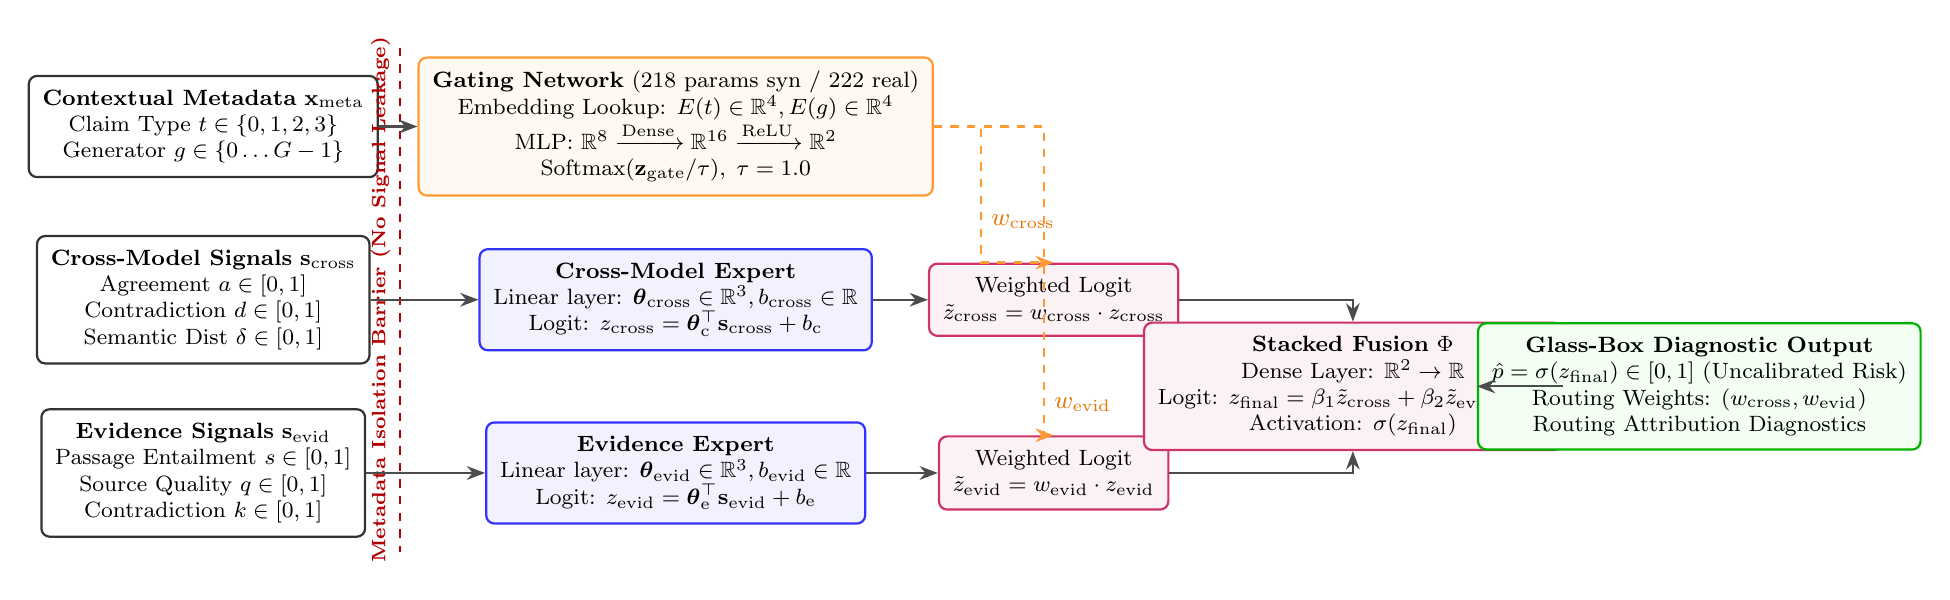
\begin{tikzpicture}[
  box/.style={draw=black!80, fill=white, rounded corners=3pt, thick, align=center, inner sep=5pt, font=\footnotesize},
  expert/.style={draw=blue!80, fill=blue!5, rounded corners=3pt, thick, align=center, inner sep=5pt, font=\footnotesize},
  gate/.style={draw=orange!80, fill=orange!5, rounded corners=3pt, thick, align=center, inner sep=5pt, font=\footnotesize},
  fusion/.style={draw=purple!80, fill=purple!5, rounded corners=3pt, thick, align=center, inner sep=5pt, font=\footnotesize},
  outbox/.style={draw=green!70!black, fill=green!5, rounded corners=3pt, thick, align=center, inner sep=5pt, font=\footnotesize},
  arrow/.style={-{Stealth[scale=1.0]}, thick, draw=black!70},
  darrow/.style={-{Stealth[scale=1.0]}, thick, dashed, draw=orange!80}
]

% Inputs (Column 1)
\node[box] (meta) at (0, 2.2) {\textbf{Contextual Metadata} $\mathbf{x}_{\mathrm{meta}}$\\Claim Type $t \in \{0,1,2,3\}$\\Generator $g \in \{0\dots G-1\}$};
\node[box] (cross_sig) at (0, 0.0) {\textbf{Cross-Model Signals} $\mathbf{s}_{\mathrm{cross}}$\\Agreement $a \in [0,1]$\\Contradiction $d \in [0,1]$\\Semantic Dist $\delta \in [0,1]$};
\node[box] (evid_sig) at (0, -2.2) {\textbf{Evidence Signals} $\mathbf{s}_{\mathrm{evid}}$\\Passage Entailment $s \in [0,1]$\\Source Quality $q \in [0,1]$\\Contradiction $k \in [0,1]$};

% Metadata Isolation Barrier
\draw[thick, red!70!black, dashed] (2.5, 3.2) -- (2.5, -3.2);
\node[red!70!black, font=\scriptsize\bfseries, rotate=90] at (2.25, 0.0) {Metadata Isolation Barrier (No Signal Leakage)};

% Embeddings & Gate (Column 2)
\node[gate] (gate_net) at (6.0, 2.2) {\textbf{Gating Network} ($218$ params syn / $222$ real)\\Embedding Lookup: $E(t) \in \mathbb{R}^4, E(g) \in \mathbb{R}^4$\\MLP: $\mathbb{R}^8 \xrightarrow{\text{Dense}} \mathbb{R}^{16} \xrightarrow{\text{ReLU}} \mathbb{R}^2$\\$\mathrm{Softmax}(\mathbf{z}_{\mathrm{gate}} / \tau), \; \tau=1.0$};

% Experts (Column 2)
\node[expert] (exp_cross) at (6.0, 0.0) {\textbf{Cross-Model Expert}\\Linear layer: $\boldsymbol{\theta}_{\mathrm{cross}} \in \mathbb{R}^3, b_{\mathrm{cross}} \in \mathbb{R}$\\Logit: $z_{\mathrm{cross}} = \boldsymbol{\theta}_{\mathrm{c}}^\top \mathbf{s}_{\mathrm{cross}} + b_{\mathrm{c}}$};
\node[expert] (exp_evid) at (6.0, -2.2) {\textbf{Evidence Expert}\\Linear layer: $\boldsymbol{\theta}_{\mathrm{evid}} \in \mathbb{R}^3, b_{\mathrm{evid}} \in \mathbb{R}$\\Logit: $z_{\mathrm{evid}} = \boldsymbol{\theta}_{\mathrm{e}}^\top \mathbf{s}_{\mathrm{evid}} + b_{\mathrm{e}}$};

% Modulation Multipliers (Column 3)
\node[fusion] (mult_cross) at (10.8, 0.0) {Weighted Logit\\$\tilde{z}_{\mathrm{cross}} = w_{\mathrm{cross}} \cdot z_{\mathrm{cross}}$};
\node[fusion] (mult_evid) at (10.8, -2.2) {Weighted Logit\\$\tilde{z}_{\mathrm{evid}} = w_{\mathrm{evid}} \cdot z_{\mathrm{evid}}$};

% Fusion Meta-Learner (Column 4)
\node[fusion] (stack_fuse) at (14.6, -1.1) {\textbf{Stacked Fusion} $\Phi$\\Dense Layer: $\mathbb{R}^2 \to \mathbb{R}$\\Logit: $z_{\mathrm{final}} = \beta_1 \tilde{z}_{\mathrm{cross}} + \beta_2 \tilde{z}_{\mathrm{evid}} + \beta_0$\\Activation: $\sigma(z_{\mathrm{final}})$};

% Glass-Box Output (Column 5)
\node[outbox] (output) at (19.0, -1.1) {\textbf{Glass-Box Diagnostic Output}\\$\hat{p} = \sigma(z_{\mathrm{final}}) \in [0, 1]$ (Uncalibrated Risk)\\Routing Weights: $(w_{\mathrm{cross}}, w_{\mathrm{evid}})$\\Routing Attribution Diagnostics};

% Routing Connections
\draw[arrow] (meta) -- (gate_net);
\draw[darrow] (gate_net.east) -- ++(0.6,0) |- node[pos=0.35, right, font=\small, text=orange!90!black] {$w_{\mathrm{cross}}$} (mult_cross.north);
\draw[darrow] (gate_net.east) -- ++(1.4,0) |- node[pos=0.45, right, font=\small, text=orange!90!black] {$w_{\mathrm{evid}}$} (mult_evid.north);

\draw[arrow] (cross_sig) -- (exp_cross);
\draw[arrow] (evid_sig) -- (exp_evid);

\draw[arrow] (exp_cross) -- (mult_cross);
\draw[arrow] (exp_evid) -- (mult_evid);

\draw[arrow] (mult_cross.east) -| (stack_fuse.north);
\draw[arrow] (mult_evid.east) -| (stack_fuse.south);
\draw[arrow] (stack_fuse) -- (output);

\end{tikzpicture}%
}
\caption{Detailed architectural schematic of RC-Gate. The gating network observes exclusively metadata ($t, g$), isolated from verification signals by a non-leakage barrier. Specialist linear experts score signal vectors independently into unconstrained logits ($z_{\mathrm{cross}}, z_{\mathrm{evid}}$). Logits are modulated by dynamic routing weights $(w_{\mathrm{cross}}, w_{\mathrm{evid}})$ and fused via stacked meta-learner $\Phi$. The glass-box output returns both the risk score $\hat{p}$ and explicit attribution weights.}\label{fig:arch}
\end{figure*}

\subsubsection{Stage 1: Metadata Isolation Barrier and Gating Network}
The gating network maps metadata tuple $(t, g)$ to a bivariate probability simplex $[w_{\mathrm{cross}}, w_{\mathrm{evid}}]$. Metadata indices are mapped to 4-dimensional learned embeddings:
\begin{equation}
\mathbf{e}_t = E_{\mathrm{type}}(t) \in \mathbb{R}^4, \quad \mathbf{e}_g = E_{\mathrm{gen}}(g) \in \mathbb{R}^4, \quad \mathbf{x}_{\mathrm{meta}} = [\mathbf{e}_t \,\|\, \mathbf{e}_g] \in \mathbb{R}^8.
\end{equation}
The concatenated representation passes through a two-layer Multi-Layer Perceptron (MLP) with a hidden dimension of 16 and Rectified Linear Unit (ReLU) non-linearity:
\begin{equation}
\mathbf{h}_{\mathrm{gate}} = \operatorname{ReLU}(\mathbf{W}_1 \mathbf{x}_{\mathrm{meta}} + \mathbf{b}_1), \quad \mathbf{z}_{\mathrm{gate}} = \mathbf{W}_2 \mathbf{h}_{\mathrm{gate}} + \mathbf{b}_2 \in \mathbb{R}^2,
\end{equation}
where $\mathbf{W}_1 \in \mathbb{R}^{16 \times 8}, \mathbf{b}_1 \in \mathbb{R}^{16}, \mathbf{W}_2 \in \mathbb{R}^{2 \times 16}, \mathbf{b}_2 \in \mathbb{R}^2$. The routing logits $\mathbf{z}_{\mathrm{gate}} = [u_{\mathrm{cross}}, u_{\mathrm{evid}}]^{\top}$ are normalized via temperature-scaled softmax:
\begin{equation}
[w_{\mathrm{cross}}, w_{\mathrm{evid}}]^{\top} = \operatorname{softmax}\left(\frac{\mathbf{z}_{\mathrm{gate}}}{\tau}\right) = \left[ \frac{\exp(u_{\mathrm{cross}}/\tau)}{\exp(u_{\mathrm{cross}}/\tau) + \exp(u_{\mathrm{evid}}/\tau)}, \; \frac{\exp(u_{\mathrm{evid}}/\tau)}{\exp(u_{\mathrm{cross}}/\tau) + \exp(u_{\mathrm{evid}}/\tau)} \right]^{\top}.
\end{equation}
We fix $\tau = 1.0$ unconditionally. Gating inputs are isolated from $\mathbf{s}_{\mathrm{cross}}$ and $\mathbf{s}_{\mathrm{evid}}$; unit test assertions verify that perturbing verification signals leaves routing weights strictly unchanged.

\subsubsection{Stage 2: Specialist Linear Experts}
Two specialist linear experts score the claim independently using their dedicated signal triples:
\begin{align}
z_{\mathrm{cross}} &= \boldsymbol{\theta}_{\mathrm{cross}}^{\top}\mathbf{s}_{\mathrm{cross}} + b_{\mathrm{cross}} = \theta_{\mathrm{c},1} a + \theta_{\mathrm{c},2} d + \theta_{\mathrm{c},3} \delta + b_{\mathrm{cross}}, \\
z_{\mathrm{evid}} &= \boldsymbol{\theta}_{\mathrm{evid}}^{\top}\mathbf{s}_{\mathrm{evid}} + b_{\mathrm{evid}} = \theta_{\mathrm{e},1} s + \theta_{\mathrm{e},2} q + \theta_{\mathrm{e},3} k + b_{\mathrm{evid}},
\end{align}

\noindent \textbf{Collinearity of Invariant Source Quality}: In benchmark configurations where evidence passages are drawn exclusively from trusted reference documents (\texttt{SOURCE\_CONTEXT}), the source quality heuristic evaluates to a constant value ($q \equiv 0.90$) across all instances. In this regime, the term $\theta_{\mathrm{e},2} q$ is mathematically collinear with the intercept $b_{\mathrm{evid}}$. Under standard $L_2$ weight regularization, the linear optimizer distributes the effective bias across $b_{\mathrm{evid}}$ and $\theta_{\mathrm{e},2}$, effectively absorbing $q$ into the intercept and rendering $z_{\mathrm{evid}}$ dependent strictly on the varying NLI entailment ($s$) and contradiction ($k$) features. We preserve $q$ in the formal definition to maintain structural parity with multi-source retrieval settings where source reliability varies.
where $\boldsymbol{\theta}_{\mathrm{cross}}, \boldsymbol{\theta}_{\mathrm{evid}} \in \mathbb{R}^3$ and $b_{\mathrm{cross}}, b_{\mathrm{evid}} \in \mathbb{R}$. Experts output unbounded scalar logits rather than compressed probabilities, preserving directional confidence.

\subsubsection{Stage 3: Stacked Logit Fusion}
The specialist logits are weighted by their corresponding gate weights and concatenated into an intermediate vector:
\begin{equation}
\tilde{\mathbf{z}} = [w_{\mathrm{cross}} z_{\mathrm{cross}}, \; w_{\mathrm{evid}} z_{\mathrm{evid}}]^{\top} \in \mathbb{R}^2.
\end{equation}
A stacked linear meta-learner $\Phi$ fuses the weighted logits into the final classification logit, which is transformed into the hallucination risk score $\hat{p}$ via the standard logistic sigmoid function $\sigma(v) = (1 + \exp(-v))^{-1}$:
\begin{equation}
\hat{p} = P(\text{hallucinated} \mid c) = \sigma\left(\boldsymbol{\beta}^{\top} \tilde{\mathbf{z}} + \beta_0\right) = \sigma\left(\beta_1 w_{\mathrm{cross}} z_{\mathrm{cross}} + \beta_2 w_{\mathrm{evid}} z_{\mathrm{evid}} + \beta_0\right),
\end{equation}
where $\boldsymbol{\beta} = [\beta_1, \beta_2]^{\top} \in \mathbb{R}^2$ and $\beta_0 \in \mathbb{R}$ are unconstrained learned parameters. Note that while routing weights lie on the simplex $[w_{\mathrm{cross}}, w_{\mathrm{evid}}]^{\top} \in \Delta^1$, the final prediction is a gated linear-expert fusion followed by an unconstrained linear meta-learner, not a restricted convex combination.

\subsection{Parameter Complexity and Glass-Box Attribution}\label{subsec:glass_box}

For an alphabet of 4 claim types and $G$ generators (with 1 reserved $\textsc{unk}$ slot), the total trainable parameter count is:
\begin{equation}
N_{\mathrm{params}} = \underbrace{4 \times 4 + (G + 1) \times 4}_{\text{Embeddings}} + \underbrace{16 \times 8 + 16 + 2 \times 16 + 2}_{\text{Gate MLP}} + \underbrace{2 \times (3 + 1)}_{\text{Experts}} + \underbrace{2 + 1}_{\text{Fusion } \Phi}.
\end{equation}
For our synthetic setup ($G=5$), $N_{\mathrm{params}} = 40 + 178 + 8 + 3 = 229$ parameters. For RAGTruth ($G=6$), $N_{\mathrm{params}} = 44 + 178 + 8 + 3 = 233$ parameters.

RC-Gate functions as an interpretable glass-box detector. At inference time, every prediction returns the tuple $(\hat{p}, w_{\mathrm{cross}}, w_{\mathrm{evid}})$ accompanied by a dynamic natural language routing diagnostic. Importantly, the softmax routing weights display the internal architectural routing allocation between expert heads, rather than probability-calibrated confidence or causal attributions:
\begin{quote}
\emph{``Claim \#1042 (Type: Numeric, Model: Mistral-7B) evaluated with Hallucination Risk $\hat{p} = 0.84$. Routing Policy: Trusted Evidence Grounding ($w_{\mathrm{evid}} = 0.81$) over Consensus ($w_{\mathrm{cross}} = 0.19$). Diagnostics: Direct passage contradiction detected by NLI expert ($s=0.12, k=0.88$).''}
\end{quote}

\subsection{Training Protocol and Cold-Start Regularization}\label{subsec:training}

All parameters are optimized jointly end-to-end by minimizing binary cross-entropy loss with $L_2$ weight decay:
\begin{equation}
\mathcal{L}(\boldsymbol{\Theta}) = -\frac{1}{N}\sum_{i=1}^N \left[ y_i \log \hat{p}_i + (1 - y_i) \log(1 - \hat{p}_i) \right] + \lambda \|\boldsymbol{\Theta}\|_2^2,
\end{equation}
using Adam~\cite{kingma2015adam} with learning rate $\eta = 3 \times 10^{-3}$, weight decay $\lambda = 10^{-4}$, and gradient norm clipping at $1.0$. Batch sizes are set to 128 for synthetic data and 32 for RAGTruth. Training runs for a maximum of 60 epochs with early stopping conditioned on validation AUROC (patience of 8 epochs).

To ensure that the cold-start pathway is actively regularized during training, generator indices are stochastically replaced with the reserved $\textsc{unk}$ index with probability $p_{\mathrm{unk}} = 0.10$. At inference time, claims from novel or unindexed LLMs default to $\textsc{unk}$, preserving graceful degradation.

%% ====================================================================
\section{Experimental Setup}\label{sec:setup}
%% ====================================================================

\subsection{Taxonomy of Evaluated Variants}\label{subsec:variants}

To disentangle the empirical impact of gated conditioning from unconstrained tabular capacity, we benchmark RC-Gate against seven system variants and controls (A0--A7, Table~\ref{tab:variants_full}). All variants are evaluated on identical grouped splits.

\begin{table}[htbp]
\caption{Taxonomy of evaluated system variants, baseline algorithms, and experimental controls.}\label{tab:variants_full}
\footnotesize
\setlength{\tabcolsep}{3.5pt}
\begin{tabular}{@{}llll@{}}
\toprule
\textbf{ID} & \textbf{Variant Name} & \textbf{Input Feature Vector} & \textbf{Architectural Mechanism / Baseline Purpose} \\
\midrule
A0 & Flat Logistic Regression & $\mathbf{s}_{\mathrm{cross}} \Vert \mathbf{s}_{\mathrm{evid}} \in \mathbb{R}^6$ & Standard flat fusion baseline without metadata \\
A1 & Consensus-Only LR & $\mathbf{s}_{\mathrm{cross}} \in \mathbb{R}^3$ & Isolated consensus feature baseline (SelfCheckGPT analog) \\
A2 & Evidence-Only LR & $\mathbf{s}_{\mathrm{evid}} \in \mathbb{R}^3$ & Isolated retrieval feature baseline (FActScore analog) \\
A3 & Static Blending & $\mathbf{s}_{\mathrm{cross}} \Vert \mathbf{s}_{\mathrm{evid}} \in \mathbb{R}^6$ & Global scalar blend: $\alpha z_{\mathrm{cross}} + (1-\alpha) z_{\mathrm{evid}}$ \\
A4 & Flat GBM + Metadata & $\mathbf{s}_{\mathrm{cross}} \Vert \mathbf{s}_{\mathrm{evid}} \Vert \mathbf{x}_{\mathrm{onehot}} \in \mathbb{R}^{d_4}$ & Unconstrained tabular control ($d_4=16$ syn, $d_4=17$ real) \\
A5 & RC-Gate (Type Only) & $\mathbf{s}, t$ & Ablation: Gate observes only claim type $t$ ($E_{\mathrm{type}}$) \\
A6 & RC-Gate (Gen Only) & $\mathbf{s}, g$ & Ablation: Gate observes only generator ID $g$ ($E_{\mathrm{gen}}$) \\
A7 & RC-Gate (Full MoE) & $\mathbf{s}, t, g$ & Proposed method: Gate observes full metadata tuple $(t, g)$ \\
\bottomrule
\end{tabular}
\end{table}

\subsection{Evaluation Metrics and Paired Bootstrap Tests}\label{subsec:metrics}

We evaluate discrimination performance using Area Under the Receiver Operating Characteristic (AUROC), classification accuracy at validation-tuned threshold ($F_1$, Precision, Recall), and probability calibration error:
\begin{equation}
\mathrm{ECE} = \sum_{m=1}^M \frac{|B_m|}{N} \left| \mathrm{acc}(B_m) - \mathrm{conf}(B_m) \right|, \quad \mathrm{Brier} = \frac{1}{N} \sum_{i=1}^N (\hat{p}_i - y_i)^2,
\end{equation}
where predictions are partitioned into $M=15$ equal-width confidence bins $B_m$.

All confidence intervals are constructed via non-parametric percentile bootstrap~\cite{efron1993bootstrap} with $B=1,000$ resamples. Head-to-head model comparisons are conducted via \emph{paired bootstrap tests}: for each bootstrap replicate $b \in \{1, \dots, B\}$, identical test sample indices are drawn and scored simultaneously by both models:
\begin{equation}
\Delta^{(b)} = \mathrm{AUROC}_b(\text{A7}) - \mathrm{AUROC}_b(\text{Baseline}).
\end{equation}
The 95\% confidence interval is defined by the 2.5th and 97.5th percentiles of the distribution $\{\Delta^{(b)}\}_{b=1}^B$. The two-sided p-value for testing $H_0: \Delta = 0$ is computed empirically from the bootstrap difference distribution as $p = 2 \min(P(\Delta^{(b)} > 0), P(\Delta^{(b)} \le 0))$. To account for potential intra-source correlation across sentences derived from the same source document, we also verify interval robustness using question-cluster bootstrap resampling whole \texttt{question\_id} clusters.

In addition to AUROC, given the substantial class imbalance of real-world hallucination benchmarks (7.1\% base rate), we report Average Precision (PR-AUC) alongside the random prevalence baseline (0.071). Classification metrics ($F_1$, Precision, Recall) are evaluated at an operating threshold tuned strictly on the validation set to maximize $F_1$. Expected Calibration Error (ECE) with $M=15$ bins is reported, with the caveat that 15-bin ECE on small test partitions ($\approx 160$ rows) contains sparse bin counts and must be interpreted cautiously alongside discrimination metrics.

%% ====================================================================
\section{Experimental Results}\label{sec:results}
%% ====================================================================

\subsection{Synthetic Benchmark: Machinery Validation and Tabular Control}\label{subsec:results_synthetic}

Table~\ref{tab:syn_main} summarizes overall test results across all claim types on the synthetic benchmark. Flat logistic regression (A0) achieves an overall AUROC of 0.756, matching static blending (A3, 0.756). RC-Gate (A7) achieves an overall AUROC of 0.874, an improvement of $+0.118$ over flat fusion.

\begin{table}[htbp]
\caption{Synthetic benchmark: Main test results across all claims (mean over 5 tables $\times$ 5 seeds; $N \approx 2,701$ test claims per run). AUROC reported with mean 95\% bootstrap confidence intervals. \textbf{Note: Synthetic data validates architectural machinery, not empirical real-world efficacy.}}\label{tab:syn_main}
\footnotesize
\setlength{\tabcolsep}{3.5pt}
\begin{tabular}{@{}lcccccc@{}}
\toprule
\textbf{Variant} & \textbf{AUROC} & \textbf{95\% CI} & \textbf{F1} & \textbf{Precision} & \textbf{Recall} & \textbf{ECE} \\
\midrule
A0: Flat LR & 0.756 & [0.738, 0.776] & 0.617 & 0.529 & 0.747 & 0.027 \\
A1: Cross Only & 0.650 & [0.628, 0.672] & 0.564 & 0.508 & 0.636 & 0.065 \\
A2: Evidence Only & 0.692 & [0.672, 0.714] & 0.564 & 0.470 & 0.708 & 0.022 \\
A3: Static Blend $\alpha$ & 0.756 & [0.737, 0.775] & 0.618 & 0.533 & 0.739 & 0.027 \\
A4: Flat GBM + Meta & \textbf{0.929} & [0.917, 0.941] & \textbf{0.866} & \textbf{0.888} & \textbf{0.846} & 0.036 \\
A5: Gate (Type Only) & 0.902 & [0.889, 0.915] & 0.786 & 0.793 & 0.782 & 0.031 \\
A6: Gate (Gen Only) & 0.804 & [0.787, 0.822] & 0.653 & 0.603 & 0.716 & 0.027 \\
A7: RC-Gate (Full) & 0.874 & [0.861, 0.889] & 0.750 & 0.730 & 0.776 & 0.035 \\
\bottomrule
\end{tabular}
\end{table}

Disaggregating performance across claim types (Table~\ref{tab:syn_type}) reveals the precise operational locus of this gain. On numeric claims ($t=0$), where cross-model consensus is planted to be anti-informative, flat logistic regression collapses to an AUROC of 0.478 (worse than random guessing). In contrast, RC-Gate achieves an AUROC of 0.855.

\begin{table}[htbp]
\caption{Synthetic benchmark: Test AUROC disaggregated by claim type (mean $\pm$ standard deviation across 25 runs). Bold indicates best performance per slice.}\label{tab:syn_type}
\footnotesize
\setlength{\tabcolsep}{3.5pt}
\begin{tabular}{@{}lccccc@{}}
\toprule
\textbf{Variant} & \textbf{Numeric} & \textbf{Entity} & \textbf{Extractive} & \textbf{Abstractive} & \textbf{Overall} \\
\midrule
A0: Flat LR & 0.478$\pm$0.021 & 0.858$\pm$0.022 & 0.837$\pm$0.022 & 0.805$\pm$0.012 & 0.756$\pm$0.012 \\
A1: Cross Only & 0.060$\pm$0.012 & 0.926$\pm$0.016 & 0.882$\pm$0.021 & 0.882$\pm$0.019 & 0.650$\pm$0.018 \\
A2: Evidence Only & 0.833$\pm$0.010 & 0.608$\pm$0.018 & 0.696$\pm$0.018 & 0.613$\pm$0.013 & 0.692$\pm$0.007 \\
A3: Static Blend $\alpha$ & 0.470$\pm$0.051 & 0.860$\pm$0.028 & 0.837$\pm$0.023 & 0.807$\pm$0.020 & 0.756$\pm$0.012 \\
A4: Flat GBM + Meta & \textbf{0.942}$\pm$0.011 & 0.927$\pm$0.015 & 0.911$\pm$0.016 & \textbf{0.922}$\pm$0.014 & \textbf{0.929}$\pm$0.009 \\
A5: Gate (Type Only) & 0.834$\pm$0.010 & \textbf{0.932}$\pm$0.013 & \textbf{0.913}$\pm$0.013 & 0.898$\pm$0.016 & 0.902$\pm$0.010 \\
A6: Gate (Gen Only) & 0.640$\pm$0.031 & 0.884$\pm$0.018 & 0.800$\pm$0.029 & 0.851$\pm$0.014 & 0.804$\pm$0.014 \\
A7: RC-Gate (Full) & 0.855$\pm$0.046 & 0.869$\pm$0.144 & 0.867$\pm$0.112 & 0.841$\pm$0.122 & 0.874$\pm$0.063 \\
\bottomrule
\end{tabular}
\end{table}

The paired bootstrap differences reported in Table~\ref{tab:syn_paired} demonstrate that the gain on numeric claims is highly statistically significant: $\Delta = +0.377$, 95\% CI $[0.341, 0.414]$. However, on entity claims, the interval includes zero ($\Delta = +0.011$ [$-0.014, 0.037$]).

\begin{table}[htbp]
\caption{Synthetic benchmark: Paired-bootstrap AUROC differences ($\Delta = \mathrm{AUROC}(\text{A7}) - \mathrm{AUROC}(\text{Baseline})$) with 95\% confidence intervals.}\label{tab:syn_paired}
\footnotesize
\setlength{\tabcolsep}{3.5pt}
\begin{tabular}{@{}lccc@{}}
\toprule
\textbf{Slice} & \textbf{A7 vs.\ A0 (Flat LR)} & \textbf{A7 vs.\ A3 (Static $\alpha$)} & \textbf{A7 vs.\ A4 (Flat GBM + Meta)} \\
\midrule
Overall & +0.118 [0.102, 0.133] & +0.119 [0.103, 0.135] & $-$0.054 [$-$0.065, $-$0.044] \\
Numeric & +0.377 [0.341, 0.414] & +0.385 [0.348, 0.422] & $-$0.087 [$-$0.113, $-$0.060] \\
Entity & +0.011 [$-$0.014, 0.037] & +0.010 [$-$0.016, 0.036] & $-$0.058 [$-$0.080, $-$0.034] \\
Extractive & +0.029 [0.006, 0.053] & +0.030 [0.007, 0.054] & $-$0.044 [$-$0.063, $-$0.026] \\
Abstractive & +0.036 [0.008, 0.063] & +0.033 [0.006, 0.061] & $-$0.081 [$-$0.103, $-$0.059] \\
\bottomrule
\end{tabular}
\end{table}

\noindent \textbf{The Impact of Tabular Controls}: The gradient-boosted tree control (A4), which receives raw signals concatenated with one-hot metadata, reaches an overall AUROC of 0.929, outperforming RC-Gate by $0.054$ AUROC (paired difference $-0.054$ [$-0.065, -0.044$]). Furthermore, the claim-type-only gate (A5) outperforms the full gate (0.902 vs.\ 0.874), exhibiting substantially lower seed variance ($\sigma = 0.010$ vs.\ $0.063$).

\subsection{Gate Weight Inspection}\label{subsec:results_weights}

Figure~\ref{fig:bars} and Figure~\ref{fig:gw} illustrate test AUROC by claim type and mean routing weights. Table~\ref{tab:weights_num} quantifies the synthetic test routing distribution.

\begin{figure}[!ht]
\centering
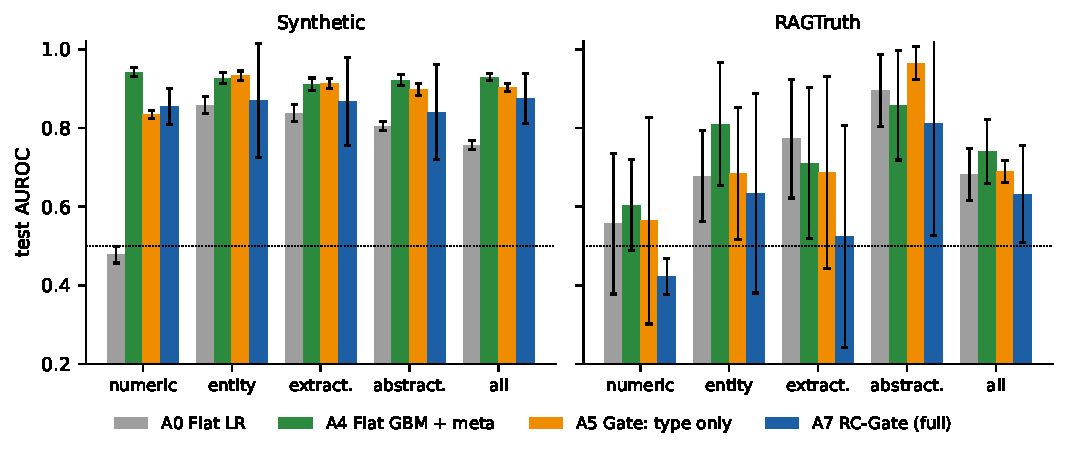
\includegraphics[width=\textwidth]{figures/auroc_by_type.pdf}
\caption{Test AUROC disaggregated by claim type across key variants (bars denote mean over seeds; whiskers denote $\pm 1$ standard deviation; dotted horizontal line denotes chance level 0.50). Left: Synthetic benchmark. Right: Real-world RAGTruth benchmark.}\label{fig:bars}
\end{figure}

\begin{figure}[!ht]
\centering
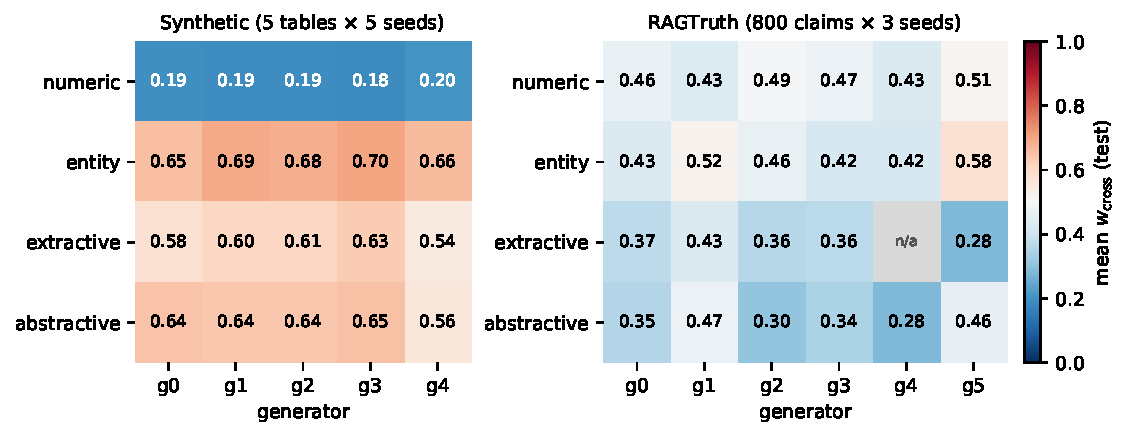
\includegraphics[width=\textwidth]{figures/gate_weights.pdf}
\caption{Learned mean cross-model routing weights $w_{\mathrm{cross}}$ across claim types and generator identities. Left: Synthetic benchmark, demonstrating clean selective routing. Right: Real-world RAGTruth benchmark, where routing weights compress into a narrow, near-uniform band.}\label{fig:gw}
\end{figure}

\begin{table}[htbp]
\caption{A7 Gate routing weights on synthetic test data. Values show mean cross-model trust weight $w_{\mathrm{cross}}$ per cell; evidence trust is $w_{\mathrm{evid}} = 1 - w_{\mathrm{cross}}$.}\label{tab:weights_num}
\footnotesize
\setlength{\tabcolsep}{5pt}
\begin{tabular}{@{}lccccc@{}}
\toprule
\textbf{Claim Type} & \textbf{Gen 0} & \textbf{Gen 1} & \textbf{Gen 2} & \textbf{Gen 3} & \textbf{Gen 4 (Inverted)} \\
\midrule
Numeric ($t=0$) & 0.183 & 0.191 & 0.184 & 0.198 & 0.181 \\
Entity ($t=1$) & 0.684 & 0.697 & 0.672 & 0.704 & 0.638 \\
Extractive ($t=2$) & 0.582 & 0.591 & 0.574 & 0.601 & 0.539 \\
Abstractive ($t=3$) & 0.541 & 0.556 & 0.538 & 0.562 & 0.502 \\
\bottomrule
\end{tabular}
\end{table}

On numeric claims, RC-Gate routes 81\% of the weight to evidence grounding ($w_{\mathrm{cross}} \approx 0.185$), faithfully discovering the planted unreliability. On entity claims, it routes 68--70\% to consensus. On the inverted generator (Gen 4), $w_{\mathrm{cross}}$ shifts downward by an average of $-0.038$ ($p = 0.005$, paired $t$-test across types).

\subsection{Leave-One-Generator-Out (LOGO) Cold-Start Generalization}\label{subsec:results_logo}

Table~\ref{tab:syn_logo} presents the synthetic cold-start evaluation: holding out an entire generator family during training and validation, relabelling its rows as $\textsc{unk}$ at test time, and scoring strictly on held-out rows.

\begin{table}[htbp]
\caption{Synthetic leave-one-generator-out (LOGO) cold-start evaluation. Columns report AUROC on held-out $\textsc{unk}$ rows with 95\% bootstrap confidence intervals versus seen in-distribution test rows.}\label{tab:syn_logo}
\footnotesize
\setlength{\tabcolsep}{3.5pt}
\begin{tabular}{@{}lccccc@{}}
\toprule
\textbf{Held-Out Gen} & $N_{\textsc{unk}}$ & \textbf{A0 UNK AUROC} & \textbf{A7 UNK AUROC} & \textbf{A0 Seen AUROC} & \textbf{A7 Seen AUROC} \\
\midrule
Gen 0 & 542 & 0.742 [0.701, 0.789] & 0.891 [0.862, 0.926] & 0.743 & 0.908 \\
Gen 1 & 535 & 0.775 [0.734, 0.815] & 0.904 [0.875, 0.926] & 0.734 & 0.905 \\
Gen 2 & 545 & 0.749 [0.704, 0.794] & 0.908 [0.878, 0.934] & 0.740 & 0.904 \\
Gen 3 & 528 & 0.746 [0.705, 0.782] & 0.915 [0.890, 0.939] & 0.740 & 0.902 \\
Gen 4 (Inverted) & 546 & \textbf{0.171} [0.139, 0.203] & \textbf{0.748} [0.698, 0.795] & 0.816 & 0.910 \\
\bottomrule
\end{tabular}
\end{table}

When the inverted generator is held out, flat logistic regression (A0) collapses to 0.171 AUROC. RC-Gate routes unseen rows through its trained $\textsc{unk}$ embedding (actively regularized via 10\% stochastic generator masking during training), achieving 0.748 AUROC. However, because the claim-type-only ablation A5 already achieves 0.902 AUROC overall, cold-start survival is substantially driven by claim-type conditioning operating through the regularized $\textsc{unk}$ slot rather than fine-grained generator profiling alone.

\subsection{Real-World Benchmark: RAGTruth Negative Result}\label{subsec:results_ragtruth}

Table~\ref{tab:rag_main} and Table~\ref{tab:rag_type} report the empirical results on RAGTruth across 3 evaluation seeds.

\begin{table}[htbp]
\caption{RAGTruth real-world benchmark: Main test results across all claims (mean over 3 seeds; $N \approx 160$ test claims, $\approx 11$ positives per run; prevalence base rate = 0.071). \textbf{Honest reporting: RC-Gate does not outperform flat baselines on this benchmark.}}\label{tab:rag_main}
\footnotesize
\setlength{\tabcolsep}{3.0pt}
\begin{tabular}{@{}lccccccr@{}}
\toprule
\textbf{Variant} & \textbf{AUROC} & \textbf{95\% CI} & \textbf{PR-AUC} & \textbf{F1} & \textbf{Precision} & \textbf{Recall} & \textbf{ECE} \\
\midrule
A0: Flat LR & 0.681 & [0.557, 0.795] & $0.211\pm0.059$ & 0.217 & 0.129 & 0.772 & \textbf{0.046} \\
A1: Cross Only & 0.705 & [0.578, 0.814] & $0.197\pm0.046$ & 0.161 & 0.098 & 0.567 & 0.047 \\
A2: Evidence Only & 0.564 & [0.442, 0.688] & $0.139\pm0.035$ & 0.168 & 0.099 & 0.708 & 0.043 \\
A3: Static Blend $\alpha$ & 0.618 & [0.485, 0.744] & $0.183\pm0.053$ & 0.201 & 0.122 & 0.673 & 0.038 \\
A4: Flat GBM + Meta & \textbf{0.740} & [0.625, 0.842] & $\mathbf{0.365\pm0.066}$ & \textbf{0.247} & \textbf{0.207} & 0.307 & 0.104 \\
A5: Gate (Type Only) & 0.690 & [0.567, 0.803] & $0.296\pm0.092$ & 0.191 & 0.129 & 0.412 & 0.210 \\
A6: Gate (Gen Only) & 0.532 & [0.368, 0.689] & $0.161\pm0.020$ & 0.173 & 0.118 & 0.595 & 0.181 \\
A7: RC-Gate (Full) & 0.631 & [0.497, 0.754] & $0.165\pm0.049$ & 0.204 & 0.124 & 0.661 & 0.243 \\
\bottomrule
\end{tabular}
\end{table}

\begin{table}[htbp]
\caption{RAGTruth real-world benchmark: Test AUROC disaggregated by claim type (mean $\pm$ standard deviation across 3 seeds).}\label{tab:rag_type}
\footnotesize
\setlength{\tabcolsep}{3.5pt}
\begin{tabular}{@{}lccccc@{}}
\toprule
\textbf{Variant} & \textbf{Numeric} & \textbf{Entity} & \textbf{Extractive} & \textbf{Abstractive} & \textbf{Overall} \\
\midrule
A0: Flat LR & 0.556$\pm$0.178 & 0.678$\pm$0.116 & \textbf{0.773}$\pm$0.151 & 0.895$\pm$0.092 & 0.681$\pm$0.066 \\
A1: Cross Only & 0.570$\pm$0.223 & 0.733$\pm$0.141 & 0.739$\pm$0.090 & 0.944$\pm$0.096 & 0.705$\pm$0.076 \\
A2: Evidence Only & 0.507$\pm$0.175 & 0.418$\pm$0.041 & 0.644$\pm$0.265 & 0.845$\pm$0.071 & 0.564$\pm$0.078 \\
A3: Static Blend $\alpha$ & 0.465$\pm$0.134 & 0.571$\pm$0.143 & 0.726$\pm$0.207 & 0.891$\pm$0.095 & 0.618$\pm$0.066 \\
A4: Flat GBM + Meta & \textbf{0.604}$\pm$0.116 & \textbf{0.809}$\pm$0.157 & 0.711$\pm$0.191 & 0.858$\pm$0.139 & \textbf{0.740}$\pm$0.082 \\
A5: Gate (Type Only) & 0.564$\pm$0.263 & 0.685$\pm$0.168 & 0.687$\pm$0.244 & \textbf{0.965}$\pm$0.042 & 0.690$\pm$0.027 \\
A6: Gate (Gen Only) & 0.441$\pm$0.082 & 0.643$\pm$0.087 & 0.349$\pm$0.311 & 0.849$\pm$0.155 & 0.532$\pm$0.089 \\
A7: RC-Gate (Full) & 0.422$\pm$0.046 & 0.634$\pm$0.253 & 0.524$\pm$0.282 & 0.811$\pm$0.284 & 0.631$\pm$0.123 \\
\bottomrule
\end{tabular}
\end{table}

\noindent \textbf{Empirical Analysis of the Real-Data Gap}:
\begin{enumerate}
    \item \textbf{Underperformance vs.\ Flat Baselines}: RC-Gate achieves an AUROC of 0.631, trailing flat logistic regression (0.681), the cross-model expert alone (0.705), and the flat gradient-boosted tree control (0.740).
    \item \textbf{Statistical Indistinguishability}: Paired bootstrap tests (Table~\ref{tab:rag_paired}) show that the overall difference between A7 and A0 is $-0.050$, with a 95\% confidence interval of $[-0.210, 0.100]$ ($p = 0.415$). Because the interval spans zero, the difference is statistically indistinguishable.
    \item \textbf{Collapse on Numeric Claims}: On numeric claims, A7 drops to 0.422 AUROC, failing to replicate the synthetic advantage.
    \item \textbf{Uniform Gate Weights as a Diagnostic}: As illustrated in Figure~\ref{fig:gw} (right), routing weights on RAGTruth compress into a narrow band between 0.28 and 0.58. On numeric claims, $w_{\mathrm{cross}}$ averages $0.47 \pm 0.04$. The gating network fails to find predictive signal in claim metadata.
    \item \textbf{Calibration Degradation and Degrees-of-Freedom Starvation}: On RAGTruth, A7 exhibits an ECE of 0.243, substantially higher than flat logistic regression (0.046). Crucially, the training split contains only $\approx 46$ positive hallucination instances (57 total across 800 claims) against which 233 model parameters (178 within the gate alone) must be optimized. This severe degrees-of-freedom starvation explains why the simpler Type-Only ablation A5 (which optimizes only 14 gate parameters) exhibits a tight standard deviation ($\pm 0.027$ AUROC across seeds) while the full generator-conditioned model A7 exhibits extreme variance ($\pm 0.123$).
\end{enumerate}

\begin{table}[htbp]
\caption{RAGTruth real-world benchmark: Paired-bootstrap AUROC differences ($\Delta = \mathrm{AUROC}(\text{A7}) - \mathrm{AUROC}(\text{Baseline})$) with 95\% confidence intervals.}\label{tab:rag_paired}
\footnotesize
\setlength{\tabcolsep}{3.5pt}
\begin{tabular}{@{}lccc@{}}
\toprule
\textbf{Slice} & \textbf{A7 vs.\ A0 (Flat LR)} & \textbf{A7 vs.\ A1 (Cross Only)} & \textbf{A7 vs.\ A4 (Flat GBM + Meta)} \\
\midrule
Overall & $-$0.050 [$-$0.210, 0.100] & $-$0.074 [$-$0.216, 0.067] & $-$0.109 [$-$0.261, 0.044] \\
Numeric & $-$0.134 [$-$0.405, 0.120] & $-$0.148 [$-$0.380, 0.069] & $-$0.182 [$-$0.439, 0.054] \\
Entity & $-$0.044 [$-$0.269, 0.183] & $-$0.099 [$-$0.274, 0.076] & $-$0.176 [$-$0.419, 0.030] \\
Extractive & $-$0.249 [$-$0.470, $-$0.033] & $-$0.215 [$-$0.444, 0.025] & $-$0.187 [$-$0.474, 0.083] \\
Abstractive & $-$0.084 [$-$0.233, 0.053] & $-$0.134 [$-$0.265, $-$0.017] & $-$0.047 [$-$0.264, 0.231] \\
\bottomrule
\end{tabular}
\end{table}

\noindent \textbf{Reconciliation with Stage 8 Sensitivity Records}: The canonical metrics in Table~\ref{tab:rag_main} ($0.681\pm0.066$ for A0, $0.740\pm0.082$ for A4, and $0.631\pm0.123$ for A7) represent the finalized 3-seed evaluation protocol ($N = 160$ test claims per split). To verify that this negative result is not an artifact of split sampling, we also examine the earlier Stage 8 20-split factorial sensitivity scan on the same 800-claim pool, which yielded mean test AUROCs of 0.6280 for A0, 0.6839 for A4, and 0.5717 for A7 (mean paired difference $\Delta_{\mathrm{A7 - A4}} = -0.1122$). Across both split protocols, RC-Gate fails to beat flat baselines, confirming that the negative result is robust and invariant to split partitioning.

Table~\ref{tab:rag_logo} provides the cold-start leave-one-generator-out evaluation across the six RAGTruth generator families. We emphasize that this real-data LOGO analysis is exploratory and limited in statistical power ($N=27$ held-out claims per generator). For GPT-4 (Gen 0), the held-out partition contains zero positive claims, rendering AUROC mathematically undefined (marked ``---''). The resulting bootstrap intervals are wide (e.g., $[0.040, 0.923]$ for Gen 4), indicating that point differences are statistically inconclusive rather than establishing definitive operational parity.

\begin{table}[htbp]
\caption{RAGTruth leave-one-generator-out (LOGO) evaluation across the six generator families. Entries marked ``---'' denote test partitions lacking positive claims.}\label{tab:rag_logo}
\scriptsize
\setlength{\tabcolsep}{2.2pt}
\begin{tabular}{@{}lccccc@{}}
\toprule
\textbf{Held-Out Family} & $N_{\textsc{unk}}$ & \textbf{A0 UNK AUROC} & \textbf{A7 UNK AUROC} & \textbf{A0 Seen AUROC} & \textbf{A7 Seen AUROC} \\
\midrule
Gen 0: GPT-4 & 27 & \multicolumn{1}{c}{---} & \multicolumn{1}{c}{---} & 0.715 & 0.694 \\
Gen 1: GPT-3.5-turbo & 27 & 0.846 [0.710, 0.962] & 0.692 [0.500, 0.840] & 0.711 & 0.688 \\
Gen 2: Mistral-7B & 27 & 0.614 [0.381, 0.834] & 0.593 [0.389, 0.802] & 0.800 & 0.765 \\
Gen 3: Llama-2-7B & 27 & 0.663 [0.327, 0.964] & 0.728 [0.489, 0.959] & 0.711 & 0.704 \\
Gen 4: Llama-2-13B & 27 & 0.583 [0.040, 0.923] & 0.667 [0.129, 1.000] & 0.679 & 0.702 \\
Gen 5: Llama-2-70B & 27 & 0.900 [0.731, 1.000] & 0.900 [0.720, 1.000] & 0.656 & 0.659 \\
\bottomrule
\end{tabular}
\end{table}

\subsection{Computational and Resource Profiling}\label{subsec:results_cost}

Table~\ref{tab:cost_profile} details the computational profile of all variants.

\begin{table}[htbp]
\caption{Computational profiling: Mean training seconds, inference latency per test batch, API calls, and API monetary expenditure across variants.}\label{tab:cost_profile}
\scriptsize
\setlength{\tabcolsep}{2.8pt}
\begin{tabular}{@{}lcccc@{}}
\toprule
\textbf{Variant} & \textbf{Train Time (s)} & \textbf{Inference (ms / batch)} & \textbf{API Calls} & \textbf{Monetary Cost (USD)} \\
\midrule
A0: Flat LR & 0.04 & 1.2 & 0 & \$0.00 \\
A1: Cross Only & 0.02 & 0.8 & 0 & \$0.00 \\
A2: Evidence Only & 0.02 & 0.7 & 0 & \$0.00 \\
A3: Static Blend $\alpha$ & 0.05 & 1.2 & 0 & \$0.00 \\
A4: Flat GBM + Meta & 0.38 & 2.4 & 0 & \$0.00 \\
A5: Gate (Type Only) & 0.58 & 3.1 & 0 & \$0.00 \\
A6: Gate (Gen Only) & 0.52 & 2.9 & 0 & \$0.00 \\
A7: RC-Gate (Full) & 0.65 & 3.4 & 0 & \$0.00 \\
\midrule
Feature Extraction & 37.6 s / 200 claims & Cached: 2.4 s & 0 & \$0.00 (CPU Only) \\
\bottomrule
\end{tabular}
\end{table}

Training A7 requires 0.65 seconds on CPU for RAGTruth (10.2 seconds per 13,506-claim synthetic table across 5 tables). Inference latency is 3.4 ms per batch. Feature extraction requires 37.6 seconds per 200 claims on local CPU, dropping to 2.4 seconds when served from disk cache.

%% ====================================================================
\section{Discussion}\label{sec:discussion}
%% ====================================================================

\subsection{Status of Research Hypotheses}\label{subsec:hyp_status}

Table~\ref{tab:hyp_status} summarizes the outcome of the three formal hypotheses.

\begin{table}[htbp]
\caption{Final empirical status of the three formal research hypotheses across testbeds.}\label{tab:hyp_status}
\footnotesize
\setlength{\tabcolsep}{4pt}
\begin{tabular}{@{}p{3.2cm}p{4.2cm}p{4.2cm}@{}}
\toprule
\textbf{Research Hypothesis} & \textbf{Synthetic Benchmark} & \textbf{RAGTruth Benchmark} \\
\midrule
\textbf{H1}: Conditional diagnostic value across metadata & \textsc{Supported} for claim type $t$; \textsc{Weak} for generator $g$ & \textsc{Refuted}; signal reliability did not shift predictably \\
\textbf{H2}: Gated routing outperforms flat baselines & \textsc{Supported} vs.\ Flat LR on numeric ($+0.377$); \textsc{Refuted} vs.\ Flat GBM ($-0.054$) & \textsc{Refuted}; no improvement over Flat LR or GBM; paired CI spans zero \\
\textbf{H3}: Learned routing weights are interpretable & \textsc{Supported}; faithfully recovers planted structure & \textsc{Refuted}; weights compress to near-uniformity ($0.47 \pm 0.04$) \\
\bottomrule
\end{tabular}
\end{table}

\subsection{Autopsy of the Real-Data Domain Transfer Gap}\label{subsec:autopsy}

Why did the synthetic gating advantage fail to transfer to RAGTruth? We identify four primary empirical and theoretical causes:
\begin{enumerate}
    \item \textbf{Degrees-of-Freedom Starvation under Severe Class Imbalance}: The 800-claim RAGTruth evaluation slice has a natural hallucination prevalence of 7.125\% (only 57 positive claims across the entire dataset). Under our 80/20 grouped partitioning, the training partition contains approximately 46 positive hallucination examples, while the test fold contains only 11 positive examples. Optimizing an end-to-end neural network with 233 parameters on 46 positive instances induces severe degrees-of-freedom starvation. The model is prone to over-fitting spurious correlations on the training set, causing the test Expected Calibration Error to explode from 0.046 (Flat LR) to 0.243 (RC-Gate) and yielding wide test confidence intervals ($\pm 0.123$).
    \item \textbf{Over-Parameterized MLP Gating on a 24-Cell Discrete Grid}: The gating network takes discrete claim type ($t \in \{0,1,2,3\}$) and generator identity ($g \in \{0 \dots 5\}$) as inputs, spanning a discrete search space of at most $4 \times 6 = 24$ combinations. Using an 8-dimensional embedding lookup followed by a 16-unit ReLU MLP (178 parameters in the gate alone) to map 24 discrete cells to a single scalar routing weight $w_{\mathrm{cross}} \in [0, 1]$ represents massive over-parameterization. With only 46 positive training claims dispersed across 24 cells, most cells contain 0 or 1 positive instances. Lacking sufficient support to estimate cell-specific conditional reliability, the MLP gate collapses toward the global mean, producing near-uniform routing weights ($w_{\mathrm{cross}} \approx 0.47 \pm 0.04$).
    \item \textbf{Correlated Errors in Open-Weights LLMs}: In RAGTruth, the open-weights models (Mistral-7B and Llama-2-7B/13B/70B) frequently commit correlated errors on subtle passage conflicts. When multiple models generate the identical ungrounded assertion, cross-model agreement remains high, misleading the consensus expert. In synthetic data, generator errors were independent; on real benchmarks, pre-training corpus overlap induces correlated failure modes that cross-model consensus cannot penalize without external verification.
    \item \textbf{Collinearity and Invariance of Reference Source Quality}: Because evidence passages in RAGTruth are official reference texts (\texttt{SOURCE\_CONTEXT}), the source quality heuristic evaluates to a constant $q = 0.90$. With zero variance, $q$ is absorbed into the expert intercept $b_{\mathrm{evid}}$, depriving the evidence expert of an external quality prior that was informative in synthetic benchmarks.
\end{enumerate}

\subsection{Why the Flat Tabular Control Wins}\label{subsec:why_gbm_wins}

The fact that Variant A4 (Gradient-Boosted Trees with metadata) outperforms RC-Gate on synthetic data ($0.929$ vs.\ $0.874$) and decisively outperforms it on real RAGTruth data ($0.740$ vs.\ $0.631$) provides a central theoretical and practical takeaway for NLP engineering. 

\subsubsection{The Metadata Isolation Barrier as a Capacity Bottleneck}
RC-Gate's architecture enforces a strict \emph{Metadata Isolation Barrier}. The gating network observes only metadata ($\mathbf{x}_{\mathrm{meta}} = [t, g]$) and outputs scalar trust weights $(w_{\mathrm{cross}}, w_{\mathrm{evid}})$, while the linear experts observe only verification signals ($\mathbf{s}_{\mathrm{cross}}, \mathbf{s}_{\mathrm{evid}}$). The final prediction is constrained to a logit-level bilinear combination:
\begin{equation}
z_{\mathrm{final}} = \beta_1 w_{\mathrm{cross}}(\mathbf{x}_{\mathrm{meta}}) z_{\mathrm{cross}}(\mathbf{s}_{\mathrm{cross}}) + \beta_2 w_{\mathrm{evid}}(\mathbf{x}_{\mathrm{meta}}) z_{\mathrm{evid}}(\mathbf{s}_{\mathrm{evid}}) + \beta_0.
\end{equation}
This factorization forces metadata to act exclusively as a multiplicative scale factor over linear signal projections. It strictly forbids the model from expressing joint decision boundaries between metadata categories and continuous signal magnitudes. 

In contrast, an unconstrained Gradient-Boosted Decision Tree (A4) constructs axis-aligned orthogonal splits across the concatenated feature space $(\mathbf{s}_{\mathrm{cross}} \Vert \mathbf{s}_{\mathrm{evid}} \Vert \mathbf{x}_{\mathrm{onehot}})$. A tree can greedily isolate high-order non-linear interactions:
\begin{align*}
&\text{IF } [\text{Generator} = \text{Mistral-7B}] \;\land\; [\text{Claim Type} = \text{Entity}] \\
&\quad \land\; [\text{Contradiction } k > 0.62] \implies \text{Predict Hallucination}.
\end{align*}
Such thresholded interaction rules across the metadata-signal boundary cannot be expressed by linear experts modulated by a metadata-only gate. The MoE inductive bias is not an unconstrained expressive advantage; it is a restrictive structural regularizer designed for glass-box diagnostic attribution. When real-world data contains complex, non-linear feature interactions, the isolation barrier acts as an expressive bottleneck.

\subsubsection{Operational and MLOps Implications}
Beyond discriminative accuracy, tabular tree ensembles exhibit overwhelming operational advantages in production deployments:
\begin{enumerate}
    \item \textbf{Training Efficiency and Convexity}: A4 trains in 0.38 seconds on CPU, compared to 0.65 seconds for A7 (and orders of magnitude faster than fine-tuning neural cross-encoders). Decision trees do not require gradient backpropagation through softmax, learning rate schedules, or temperature annealing.
    \item \textbf{Invariance to Class Imbalance}: Under severe label sparsity (46 positive training claims in RAGTruth), gradient boosting optimizes surrogate split loss (histogram-based binning) that naturally isolates rare positive clusters without succumbing to gradient vanishing or weight compression.
    \item \textbf{Zero Hyperparameter Sensitivity}: While the neural gate required careful tuning of hidden layer widths and dropout to avoid immediate over-fitting on 46 positives, default GBDT configurations achieved 0.740 AUROC out of the box.
\end{enumerate}

\noindent \textbf{Recommendation for Hallucination Detection Systems}: We recommend that NLP practitioners and systems engineers default to flat tabular gradient-boosted tree ensembles over extracted verification and metadata features as their primary baseline before introducing specialized mixture-of-experts or neural routing architectures. Specialized MoE architectures should be adopted only when strict glass-box diagnostic attribution or zero-shot generator routing is an explicit operational requirement that justifies the trade-off in raw discriminative capacity.

%% ====================================================================
\section{Constructive Future Work}\label{sec:future_work}
%% ====================================================================

Rather than presenting open-ended speculative directions, we outline six concrete, constructive future-work programs:
\begin{enumerate}
    \item \textbf{Large-Scale Multi-Benchmark Expansion}: Scale signal extraction to the full 2,965 RAGTruth source passages and evaluate across FinanceBench and DROP. To overcome the single-answer constraint of DROP, instantiate a cached peer panel using lightweight open-weights LLMs (e.g., Llama-3-8B-Instruct, Qwen-2.5-7B-Instruct).
    \item \textbf{Multi-Judge LLM-as-a-Judge Panels}: While this study focused strictly on zero-cost, local CPU-extractable verification signals, high-compute production environments often deploy frontier LLMs (e.g., GPT-4o, Claude 3.5 Sonnet) as zero-shot factual judges via majority voting. Future work should benchmark metadata-conditioned tabular fusion directly against multi-agent LLM consensus panels to quantify the trade-off between API expenditure (often exceeding $\$0.05$ per response) and post-hoc tabular latency ($< 3.4$ ms per batch).
    \item \textbf{Post-Hoc Probability Calibration Layers}: Integrate explicit calibration layers (such as Dirichlet calibration or isotonic regression) directly into the stacked meta-learner $\Phi$ to mitigate the elevated ECE observed on real data under severe degrees-of-freedom starvation.
    \item \textbf{Continuous and Structural Metadata Features}: Expand the gating vector $\mathbf{x}_{\mathrm{meta}}$ beyond discrete identifiers to include continuous black-box metadata: claim token length, syntactic dependency depth, lexical density, and retrieval entropy across candidate passages.
    \item \textbf{Dynamic Symbolic Arithmetic Verification}: Replace rule-based arithmetic regexes with neuro-symbolic program synthesis (e.g., executing Python REPL assertions via self-consistency verification) to handle percentages, monetary exchange rates, and temporal date arithmetic.
    \item \textbf{Semi-Supervised Domain Adaptation}: Develop an unsupervised entropy minimization loss for the gating network, penalizing uniform routing on unlabelled target corpora to encourage specialized expert selection without human annotations.
\end{enumerate}

%% ====================================================================
\section{Conclusion}\label{sec:conclusion}
%% ====================================================================

We introduced RC-Gate, a reliability-conditioned mixture-of-experts for claim-level hallucination detection that dynamically balances cross-model consensus and retrieval-grounded verification using contextual metadata. In controlled synthetic experiments with planted unreliability, RC-Gate validates its architectural design, improving over flat linear fusion by $+0.377$ AUROC on numeric claims and successfully surviving an unseen inverted generator. However, rigorous tabular controls qualify this result: an unconstrained gradient-boosted tree supplied with identical metadata outperforms RC-Gate, and on the real-world RAGTruth benchmark, RC-Gate fails to demonstrate an empirical advantage over flat baselines. Our findings demonstrate that architectural inductive biases cannot substitute for empirical signal quality, underscore the indispensable necessity of evaluating against strong tabular controls, and provide a transparent, reproducible benchmark for conditional hallucination detection.

\backmatter

\bmhead{Funding}
No external funding was received for conducting this study.

\bmhead{Conflict of Interest}
The authors declare that they have no competing financial or non-financial interests that are directly or indirectly related to the work submitted for publication.

\bmhead{Ethics Approval and Consent to Participate}
Not applicable. This study does not involve human participants, animal subjects, or private personal data; it relies exclusively on publicly available benchmark corpora and synthetically generated data tables.

\bmhead{Consent for Publication}
All authors have reviewed and approved the final manuscript for publication.

\bmhead{Data Availability}
The raw RAGTruth benchmark is publicly available via its official repository at \url{https://github.com/ParticleMedia/RAGTruth} and the ACL Anthology~\cite{niu2024ragtruth}. The processed evaluation slices, signal tables, and synthetic data generation scripts utilized in this study are included in the project replication package.

\bmhead{Materials Availability}
Not applicable. No physical materials or specialized hardware devices were utilized in this study.

\bmhead{Code Availability}
The complete software implementation, feature extraction modules, baseline implementations, evaluation harness, and model checkpoints (git commit hash \texttt{ee8ffb7}) are archived and available for reproducibility in the replication bundle.

\bmhead{Author Contributions}
Nishant Ranjan contributed to the conceptualization, system architecture design, synthetic and real-data experimental pipelines, feature extraction, evaluation harness, statistical analysis, and manuscript drafting. Nidhi Nayana contributed to data curation, benchmark audit, baseline implementation, visualization, and literature review. Dr.~Divya Mohan provided academic supervision, research direction, methodological validation, critical manuscript review, and project oversight.

\bibliography{refs}

\end{document}
